\documentclass[11pt]{article}

\usepackage[margin=1in]{geometry}
\usepackage[T1]{fontenc}
\usepackage[utf8]{inputenc}
\usepackage{lmodern}
\usepackage{microtype}
\usepackage{amsmath,amssymb,amsthm,mathtools}
\usepackage{bm}
\usepackage{booktabs}
\usepackage{multirow}
\usepackage{array}
\usepackage{longtable}
\usepackage{tabularx}
\usepackage{enumitem}
\usepackage{xcolor}
\usepackage{graphicx}
\usepackage{float}
\usepackage{hyperref}
\usepackage[nameinlink,noabbrev]{cleveref}

\hypersetup{
  colorlinks=true,
  linkcolor=blue,
  citecolor=blue,
  urlcolor=blue
}

\newtheorem{definition}{Definition}
\newtheorem{theorem}{Theorem}
\newtheorem{corollary}{Corollary}
\newtheorem{proposition}{Proposition}
\newtheorem{lemma}{Lemma}
\newtheorem{remark}{Remark}

\title{Representation-Dependent Recoverability and a Fourier-Layer Separation in Quantum Compilation}
\author{}
\date{}

\begin{document}

\maketitle

\begin{abstract}
Quantum circuit lowering preserves unitary semantics, but it can change which
resource-reducing structures remain recoverable by a bounded compiler. We
identify this phenomenon as a \emph{representation-dependent recoverability
gap}: after a circuit is materialized into a flat target-basis stream,
globally meaningful phase, repetition, or conjugation structure may become
locally indistinguishable, while a semantic term representation can keep the
same structure explicit until after aggregation and candidate selection.

The main result is a Fourier-layer recoverability separation. For
$C_{m,r}=H_{\Lambda}D_m(\boldsymbol{\theta})^rH_{\Lambda}$, where
$D_m$ is a commuting diagonal phase layer, a restricted bounded flat compiler
that cannot reconstruct a global phase-polynomial representation must retain
$\Omega(rm)$ nontrivial lowered phase-gadget structure. A pre-basis semantic
compiler aggregates the commuting coefficients and emits $O(m)$ structure; in
the fixed-width case this becomes an $\Omega(r)$ versus $O(1)$ separation. The
theorem is a restricted-class separation rather than a universal lower bound:
it identifies the boundary between flat post-lowering recovery and semantic
global lifting.

We test the principle in UCC as an experimental artifact: a bounded semantic
term controller with Fourier-layer, repeated, inverse, mirrored, and
conjugation terms. The evidence role split is deliberate. Fourier-layer circuits
provide the primary separation witness; mirrored and conjugation circuits
provide secondary anti-regression evidence by restoring parity with strong flat
optimizers on Grover-like structures. On the canonical fixed-width
$H D^r H$ witness, the semantic artifact reduces inputs of approximately
$4$k, $10$k, $20$k, $50$k, and $100$k gates to $42$ gates, depth $24$, and
$12$ \texttt{cx} gates, while \texttt{qiskit opt3} grows to $9{,}588$,
$23{,}988$, and $47{,}988$ gates at the first three sizes and times out at
$50$k and $100$k. A generalized fixed-width suite varies the diagonal topology
and angle family at $n=4$ and gives $42/42$ strict structural-quality wins over
\texttt{qiskit opt3}; semantic UCC completes every comparable point, while
\texttt{qiskit opt3} times out on $14$ of them. A Fourier-layer ablation removes
this completed constant-output recovery, and a resource-consequence experiment
shows that, under a rotation-count Clifford+$T$ proxy at precision $10^{-10}$,
semantic-first compilation keeps a constant $T$-proxy of $2{,}200$, whereas
materialize-first \texttt{qiskit opt3} grows from $479{,}300$ to
$2{,}399{,}300$ before timing out.
\end{abstract}

\section{Introduction}

Quantum circuit compilation is representation-sensitive. The usual
lower-then-optimize pipeline first decomposes high-level algorithmic structure
into a target basis and then optimizes the resulting instruction stream. This
lowering map is semantically exact, but semantic exactness does not imply that
optimization evidence remains locally recoverable. Repeated phase ladders,
commuting diagonal layers, inverse shells, and mirrored conjugations can become
distributed across a large basis-level materialization in which their original
boundaries are no longer locally evident.

The bottleneck studied here is not the computational power of an unrestricted
optimizer, but the \emph{recoverability} of structure under the representation
available to a bounded compiler. A flat basis-level compiler with bounded local
evidence observes only small neighborhoods of the materialized stream. When a
structured family contains many repeated interior positions with identical
local certificate profiles, such a compiler cannot safely select the globally
meaningful aggregation or cancellation boundaries without extra semantic
information. A semantic compiler avoids this ambiguity by keeping the relevant
terms explicit before basis materialization.

The conceptual point is an information-locality one. Two representations can
describe the same unitary while exposing different certificates to a bounded
compiler. A high-level diagonal term carries its Pauli support and coefficient
as explicit data; after target-basis lowering, the same term may be dispersed
into a repeated pattern whose local neighborhoods collide with many other
interior positions. Recoverability therefore depends not only on the unitary,
but also on the representation in which the optimizer is asked to act.

We distinguish two operational regimes of this recoverability gap. The first is
\emph{structural separation}: a semantic representation exposes a global
aggregation, such as coefficient addition in a commuting Fourier layer, that a
restricted flat compiler cannot recover without reconstructing a global
diagonal representation. Our main theorem proves this regime for
$C_{m,r}=H_{\Lambda}D_m(\boldsymbol{\theta})^rH_{\Lambda}$, giving an
$\Omega(r)$ versus $O(1)$ fixed-width separation in retained phase-gadget
structure. The second regime is \emph{recoverability parity}: semantic lifting
does not beat every strong flat compiler, but it prevents catastrophic
regression by preserving high-level identities such as mirrored or conjugation
shells. These two regimes let the paper separate its primary scientific
witness from broader anti-regression evidence.

UCC is used as the artifact and diagnostic testbed for this principle. Its
default flow is composable across frontends and backends, but that
composability also makes it vulnerable to structured-circuit regressions. The
artifact adds a bounded semantic term algebra, dispatch-driven candidate
control, projected block selection, late materialization, and cache-aware
reuse. On the primary Fourier-layer witness, the semantic path produces the
predicted constant output while tested flat pipelines grow or time out. On
mirrored and conjugation families, it restores UCC to \texttt{qiskit opt3}-level
quality rather than claiming a new external-baseline separation.

The remainder of the paper is organized as follows.
\Cref{sec:related} positions the work relative to prior literature.
\Cref{sec:problem,sec:method,sec:integration} define the recoverability
problem, the bounded semantic term algebra, and the UCC integration.
\Cref{sec:experimental-setup,sec:results} present the experimental protocol
and results. \Cref{sec:discussion,sec:threats,sec:reproducibility,sec:conclusion}
discuss limitations, validity threats, reproducibility, and conclusions.

\section{Related Work}
\label{sec:related}

Our work is best understood as a representation-aware compilation study. The
central distinction is between two compiler regimes: semantic representations
that explicitly encode algebraic structure, and flat post-lowering pipelines
that attempt to recover structure from a target-basis instruction stream. UCC
is the systems artifact used to test this distinction; it is not the main
scientific object. The paper is therefore related to, but distinct from, prior
work in semantic circuit representations, architecture-aware compilation,
benchmark design, and open compiler infrastructure.

A first relevant line of work studies semantic representations for circuit
simplification. ZX-calculus-based simplification has shown that alternative
circuit representations can expose reductions that are difficult to recover
from a gate-level instruction sequence alone~\cite{duncan2020zx}. Phase
polynomial and diagonal representations play a similar conceptual role for
commuting phase structure: they preserve coefficients and supports that can be
hard to infer after full basis materialization. Our Fourier-layer theorem
formalizes this distinction for a restricted flat-recovery class. A compiler
that explicitly reconstructs a global ZX, phase-polynomial, or diagonal IR is
not a counterexample to our lower bound; it belongs to the semantic side of the
separation.

A second related direction emphasizes that compilation outcomes depend strongly
on pipeline strategy and preprocessing decisions. Architecture-aware
compilation via lazy synthesis, for example, shows that decomposition, routing,
and synthesis choices can materially affect final gate count and
depth~\cite{martiel2022lazy}. Our setting differs in target: we focus on
pre-basis recoverability of algebraic structure rather than routing under
connectivity constraints. The broader lesson is aligned: once a representation
choice has destroyed useful structure, later local optimization may not be able
to recover it cheaply.

Benchmark design is also central to the paper, but benchmarks play different
roles in our argument. The fixed-width $H D^r H$ family is a minimal theorem
witness, analogous to a separating family: it isolates whether commuting
diagonal phase structure is aggregated before materialization. Official Qiskit
instances, \texttt{MQT Bench}, and \texttt{SupermarQ} cases are natural-source
controls and anti-regression tests. Public benchmark work argues that quantum
software tools should be evaluated on practical benchmark suites to improve
comparability and transparency~\cite{quetschlich2023mqtbench}; holistic
benchmarking work further argues that meaningful performance assessment often
requires studying the full stack, including compilation strategy and hardware
effects~\cite{mills2021holistic}. Related full-stack resource studies likewise
emphasize that cross-layer optimization choices can dominate overall system
efficiency~\cite{fellousasiani2023mnr}.

Finally, our paper fits within the line of work that treats compiler
infrastructure and specialized compiler flows as publishable research artifacts.
Open-source compiler frameworks established the value of extensible toolchains
with optimization plug-ins, synthesis passes, and hardware-targeting
components~\cite{steiger2018projectq}. More recent compiler papers have also
shown that architecture-specific compiler systems are well within
scope~\cite{kreppel2023shuttling,tan2024dpqa,watkins2024surfacecode}. Our
claim is narrower than universal compiler dominance: UCC is the artifact used to
test a representation principle, with Fourier layers as the primary separation
witness and mirrored/conjugation shells as secondary parity-recovery evidence.

\section{Contributions}

This paper is built around one central claim: representation choice can create
an asymptotic gap in the recoverability of quantum-circuit structure. The claim
is intentionally falsifiable: a compiler that reconstructs a global
phase-polynomial, ZX, or commuting-diagonal representation belongs to the
semantic side of the theorem rather than contradicting it. The contributions
are:

\begin{enumerate}[leftmargin=1.5em]
    \item \textbf{Recoverability framework.} We formalize representation-dependent recoverability and define a restricted class of locally certifying bounded flat compilers. A certificate-collision lemma explains why repeated semantic positions can become locally indistinguishable after lowering.
    \item \textbf{Fourier-layer separation.} We prove the primary separation: under explicit bounded-local recovery assumptions, $H_{\Lambda}D_m(\boldsymbol{\theta})^rH_{\Lambda}$ requires $\Omega(rm)$ retained lowered phase-gadget structure for restricted flat recovery but only $O(m)$ structure for pre-basis semantic phase aggregation, with an $\Omega(r)$ versus $O(1)$ fixed-width corollary.
    \item \textbf{Semantic compilation artifact.} We instantiate the principle in UCC through a bounded semantic term algebra with Fourier-layer, repeated, inverse, mirrored, and conjugation terms; projected cost comparison; late materialization; cache-aware subterm reuse; and conservative backend-aware dispatch.
    \item \textbf{Evidence chain.} We connect the theorem to mechanism and scope through the fixed-width Fourier witness, external pipeline diagnostics, Fourier ablation, resource estimates, algorithmic-source controls, mirrored/conjugation anti-regression cases, and finite-seed hardware-aware stability checks.
\end{enumerate}

\section{Problem Definition}
\label{sec:problem}

Let a high-level quantum circuit be represented as a finite instruction sequence
\[
C = (g_1, g_2, \dots, g_m),
\]
where each instruction $g_i$ carries an operation type, normalized parameter tuple, quantum operand tuple, and classical operand tuple. Let $\mathcal{L}_B(\cdot)$ denote lowering into a fixed target basis $B$, and let $\mathcal{P}_{\mathrm{ucc}}(\cdot)$ denote the default downstream UCC compilation flow after lowering.

We are interested in structured circuits containing one or more of the following higher-level structures:
\begin{enumerate}[leftmargin=1.5em]
    \item exact inverse blocks: $U U^\dagger$,
    \item repeated blocks and repeated dominant prefixes: $B^r = B B \cdots B$,
    \item phase-ladder or Fourier-type layers built from alternating Hadamards, commuting diagonal phase operations, and terminal swaps,
    \item mirrored or self-inverse shells whose expanded instruction groups are symmetric under reversal and involution.
\end{enumerate}

The paper studies the following question:

\begin{quote}
Given a high-level circuit $C$, can a bounded preprocessing pass produce a simplified circuit $C'$ that preserves semantics while exposing structure that would otherwise be lost during basis lowering?
\end{quote}

The key distinction is between:
\begin{itemize}[leftmargin=1.5em]
    \item \textbf{gate-set translation overhead}, which is expected when lowering to a new target basis, and
    \item \textbf{missed structural simplification}, which occurs when the pipeline fails to exploit structure that is available before lowering.
\end{itemize}

\begin{definition}[Stable signature]
For an instruction $g$, define its \emph{stable signature}
\[
\sigma(g) := (\mathrm{name}(g), \mathrm{params}(g), \mathrm{qargs}(g), \mathrm{cargs}(g)),
\]
where parameters are normalized into a canonical numeric representation and operand lists are recorded in a fixed order. For a block $U = (g_i,\dots,g_j)$, define
\[
\sigma(U) := (\sigma(g_i),\dots,\sigma(g_j)).
\]
\end{definition}

\begin{definition}[Pre-basis structural opportunity]
A \emph{pre-basis structural opportunity} in a circuit $C$ is a rewrite or candidate reduction that is detectable from a high-level semantic view of $C$ but is not guaranteed to remain detectable after applying $\mathcal{L}_B$. Typical examples include exact inverse blocks, repeated blocks, phase-ladder layers, mirrored/self-inverse shells, and dominant repeated prefixes.
\end{definition}

\begin{definition}[Structural regression]
Let $\kappa(\cdot)$ be a structural cost measure, for example a tuple consisting of total gate count, depth, and two-qubit gate count under a fixed tie-breaking rule. We say that the default compilation flow exhibits a \emph{structural regression} on input $C$ if
\[
\kappa\!\left(\mathcal{P}_{\mathrm{ucc}}(\mathcal{L}_B(C))\right)
>
\kappa(\widetilde{C}),
\]
for some semantically equivalent candidate $\widetilde{C}$ obtainable from $C$ by bounded pre-basis structural preprocessing followed by the same target basis protocol.
\end{definition}

This definition is intentionally operational rather than universal: the paper does not claim that all useful structure can be characterized in closed form, only that some important classes of structure can be identified early enough to prevent avoidable regressions.

\begin{figure*}[t]
\centering
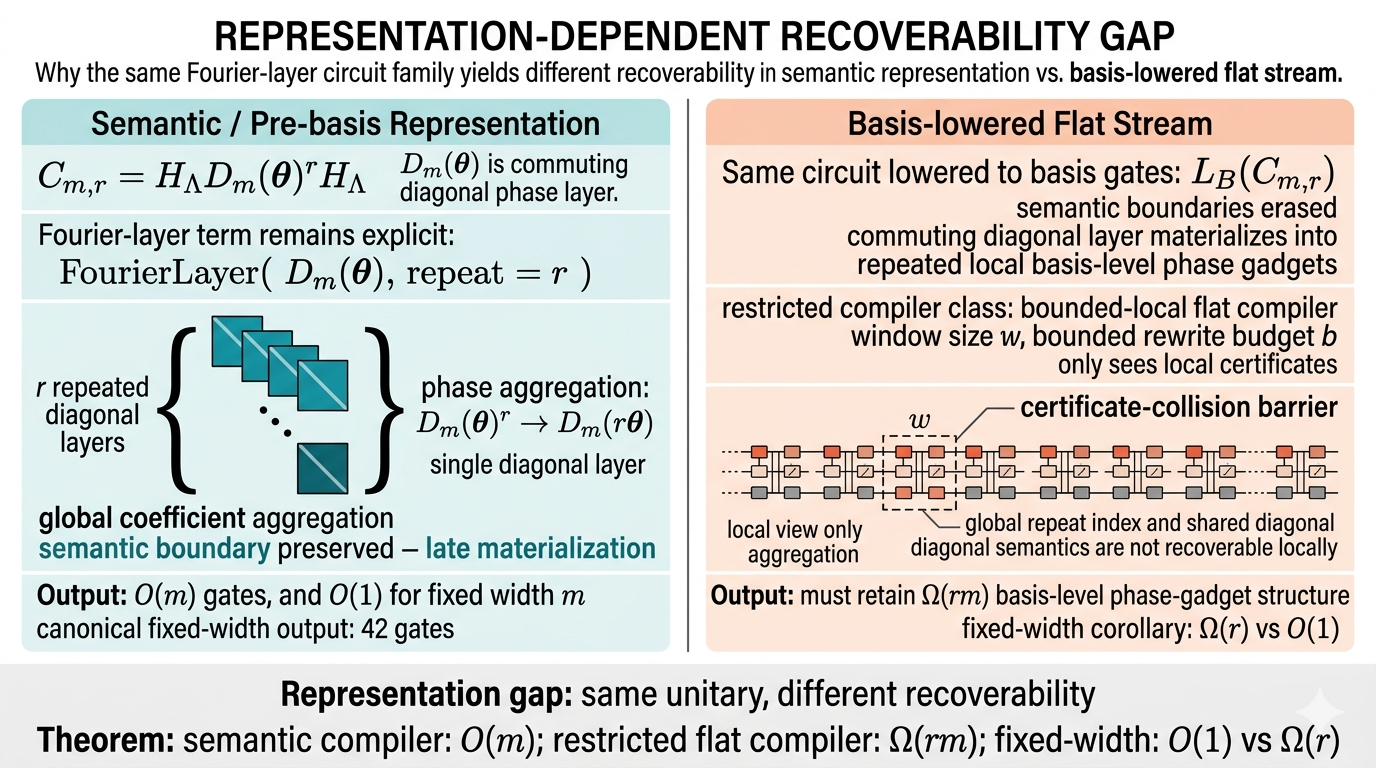
\includegraphics[width=\textwidth]{../Graph Materials/conceptual_theorem_figure.png}
\caption{Representation-dependent recoverability gap for the fixed-width Fourier-layer witness. A semantic pre-basis representation preserves the repeated commuting diagonal layer and aggregates coefficients before materialization, giving an $O(m)$ output and an $O(1)$ fixed-width corollary. A basis-lowered flat stream erases semantic boundaries, so a bounded-local flat compiler that does not reconstruct a global diagonal representation must retain repeated basis-level phase-gadget structure.}
\label{fig:recoverability-gap}
\end{figure*}

\section{Method}
\label{sec:method}

\Cref{fig:recoverability-gap} shows the representation distinction that the
artifact implements: semantic structure is preserved long enough to support
global phase aggregation, whereas early basis lowering can leave only repeated
local certificates available to a bounded flat compiler.

\subsection{Compilation Principle}

The artifact implements a representation principle:
\begin{quote}
if exploitable structure is easier to preserve, compare, or reuse before basis
lowering than after it, then compilation should first move that circuit into a
bounded semantic term algebra and postpone flat materialization until after
candidate selection.
\end{quote}

This principle is motivated by a representation-dependent notion of
recoverability. Basis lowering preserves semantics, but it does not necessarily
preserve the cheap detectability of repeated blocks, inverse blocks,
Fourier-like phase ladders, or mirrored/self-inverse shells. In that sense,
lowering is semantics-preserving but not automatically
opportunity-preserving.

\subsection{Representation Gap and Recoverability Gap}

The theoretical claim behind the artifact is representation-dependent
recoverability. Let:
\begin{itemize}[leftmargin=1.5em]
    \item $L_B(C)$ be lowering into target basis $B$,
    \item $\kappa$ be a conservative structural cost,
    \item $\mathcal{T}_K(C)$ be the bounded set of semantic candidates produced by the semantic lift under budget $K$,
    \item $\mathfrak{A}_w$ be a bounded post-lowering compiler class restricted to flat basis-level candidate generation or local rewrite regimes.
\end{itemize}

For the sharper family statements below, we replace the earlier informal
boundary-oblivious shorthand by a more explicit restricted class
$\mathfrak{F}^{\mathrm{lc}}_{w,b,\rho}$ of \emph{locally certifying bounded
flat compilers}. A compiler in $\mathfrak{F}^{\mathrm{lc}}_{w,b,\rho}$
operates only on fully materialized basis-level circuits, observes
neighborhoods of radius at most $w$, generates at most $b$ bounded candidates,
and may recover a semantic unit only across boundaries admitting a local
certificate built from at most $\rho$ radius-$w$ witness windows. Write
$\mathrm{cert}(\partial, L_B(C))$ for the certificate profile attached to a
candidate boundary $\partial$, and let
$\mathrm{mult}(\mathrm{cert}(\partial, L_B(C)))$ denote the number of
boundaries with the same certificate profile. The class is
\emph{collision-respecting}: if
$\mathrm{mult}(\mathrm{cert}(\partial, L_B(C))) = \Theta(r)$, then the
compiler may not use that certificate to single out one repeated interior
boundary as a uniquely recoverable semantic boundary. Only
$O(1)$-multiplicity certificates may justify singling out a boundary.

For the sharper lower-bound-style statements below, we also assume that the
certificate map factors through a finite witness alphabet induced by the
at-most-$\rho$ radius-$w$ witness windows and a bounded internal state, and
that away from an $O(1)$ anomaly zone this certification rule is
translation-invariant on the lowered repeated body.

Define the $(K,w)$-representation gap of $C$ by
\[
\mathrm{Gap}^{K,w}_{\mathrm{rep}}(C)
:=
\inf_{A \in \mathfrak{A}_w} \kappa(A(L_B(C)))
-
\inf_{T \in \mathcal{T}_K(C)} \kappa(L_B(T)).
\]
Define the operational recoverability gap by
\[
\mathrm{Gap}^{K,w}_{\mathrm{rec}}(C)
:=
\kappa(C_{\mathrm{flat}}^\star) - \kappa(C_{\mathrm{term}}^\star),
\]
where $C_{\mathrm{flat}}^\star$ is the best candidate recovered from the flat
basis-lowered representation and $C_{\mathrm{term}}^\star$ is the best candidate
recovered from the bounded semantic term representation.

The meaning is simple: semantics may survive lowering, while cheap
recoverability of the opportunity may not. This is the sense in which the
artifact is representation-aware rather than a better default pass schedule.

\begin{lemma}[Certificate-collision lower bound]
\label{lem:certificate-collision}
Let $C_r$ be a repeated family with $\Theta(r)$ interior semantic boundaries.
Suppose that:
\begin{enumerate}[leftmargin=1.5em]
    \item every compiler in $\mathfrak{F}^{\mathrm{lc}}_{w,b,\rho}$ uses the finite-alphabet, translation-invariant certification rule above,
    \item for every interior boundary $\partial$,
\[
\mathrm{mult}(\mathrm{cert}(\partial, L_B(C_r))) = \Theta(r).
\]
\end{enumerate}
Then every compiler in $\mathfrak{F}^{\mathrm{lc}}_{w,b,\rho}$ can certify at
most $O(1)$ boundaries of $L_B(C_r)$.
\end{lemma}

This lemma is the lower-bound-style bottleneck used by the family theorems
below: the flat compiler is not blocked because semantics disappear, but
because all interior boundaries are locally ambiguous and the class is
forbidden to break that ambiguity by bounded, translation-invariant local
evidence.

\subsection{Primary Theorem: Fourier-Layer Recoverability Separation}

The central formal statement is not about inverse cancellation. It is a
non-inverse Fourier-layer separation in which the exploitable structure is
Abelian phase aggregation. This is the paper's primary theorem: it provides a
clean witness that semantic pre-basis compilation and bounded flat
post-lowering recovery can have different asymptotic power on the same unitary
family.

For the separation statement, write $\operatorname{pg}_B(C)$ for the number of
nontrivial bounded-arity phase-gadget atoms retained after lowering to the
fixed target basis $B$. This is a structural measure rather than a claim about
one specific syntactic gate sequence. Under any fixed bounded-arity lowering
convention, each retained nontrivial phase gadget contributes at least a
constant amount of target-basis structure, so lower bounds on
$\operatorname{pg}_B$ imply the corresponding asymptotic lower bounds for gate
count and two-qubit count up to constant factors.

Let
\[
D_m(\boldsymbol{\theta})
:=
\prod_{j=1}^{m} \exp\!\left(-i\theta_j P_j/2\right),
\]
where each $P_j$ is a diagonal Pauli-$Z$ string or a bounded-arity diagonal
phase interaction, and all $P_j$ commute. Define
\[
C_{m,r}
:=
H_{\Lambda}\,D_m(\boldsymbol{\theta})^r\,H_{\Lambda},
\]
where $H_{\Lambda}$ is a fixed layer of Hadamards on the qubits touched by the
Fourier layer. This is a non-inverse family: there is no adjacent
$U U^\dagger$ cancellation. The only algebraic opportunity is that the
diagonal factors commute and repeated coefficients can be added before basis
materialization.

\begin{definition}[Fourier-layer semantic compiler]
A compiler is a \emph{Fourier-layer semantic compiler} on $C_{m,r}$ if, before
lowering to the target basis, it represents $D_m(\boldsymbol{\theta})$ as a
commuting diagonal phase-polynomial object and applies the coefficient
aggregation rule
\[
D_m(\boldsymbol{\theta})^r
=
\prod_{j=1}^{m}
\exp\!\left(-i(r\theta_j)P_j/2\right)
\]
up to the chosen global-phase convention and parameter normalization.
\end{definition}

\begin{definition}[Basis-local compiler for the Fourier-layer family]
Fix constants $w,b,\rho$. A compiler belongs to
$\mathfrak{F}^{\mathrm{fl}}_{w,b,\rho}$ on the family $C_{m,r}$ if it receives
only the fully basis-lowered stream $L_B(C_{m,r})$ and not the semantic
provenance of the repeated diagonal terms. It may apply arbitrary
unitarity-preserving local basis identities, bounded commutations, bounded
peephole rewrites, and at most $b$ bounded candidate-generation rounds. However,
any rewrite whose effect is to fuse repeated occurrences of a phase term, or a
bounded cluster of phase terms, must be justified by a certificate built from
at most $\rho$ radius-$w$ windows of the target-basis stream. The certificate
must authorize the specific local fusion or bounded cluster being rewritten; a
repeated local certificate profile cannot by itself authorize a bulk global
aggregation over all copies. The compiler is not allowed to construct an
auxiliary representation keyed by global Pauli strings, global phase-polynomial
terms, or commuting-diagonal Hamiltonian terms before performing the fusion.
As above, the certification rule is finite-alphabet, translation-invariant
away from an $O(1)$ prefix/suffix anomaly zone, and collision-respecting.
\end{definition}

The following theorem is therefore a restricted-class separation. It should
not be read as a lower bound against compilers that first reconstruct a global
phase-polynomial, ZX, or diagonal-Hamiltonian representation; such compilers
belong to the semantic side of the separation.

\begin{theorem}[Fourier-layer recoverability separation]
\label{thm:fourier-layer-separation}
Fix constants $w,b,\rho$ and a fixed bounded-arity target-basis lowering
scheme $L_B$. Consider
$C_{m,r}=H_{\Lambda}D_m(\boldsymbol{\theta})^rH_{\Lambda}$ with $m>w$. Assume:
\begin{enumerate}[leftmargin=1.5em]
    \item \textbf{bounded arity:} every $P_j$ has support bounded independently of $m$ and $r$;
    \item \textbf{non-resonance:} for the repetition range under consideration, $r\theta_j\not\equiv 0 \pmod{2\pi}$ for every non-removable term $P_j$; for an asymptotic family this is satisfied, for example, by choosing $\theta_j/\pi$ irrational;
    \item \textbf{periodic separated lowering:} in the interior of $L_B(C_{m,r})$, two consecutive occurrences of the same semantic phase term $P_j$ are separated by one full period containing $\Theta(m)$ other lowered phase gadgets, and the radius-$w$ witness neighborhoods around interior occurrences of the same $P_j$ are identical up to translation;
    \item \textbf{bounded local recovery:} the compiler is in $\mathfrak{F}^{\mathrm{fl}}_{w,b,\rho}$, so fusing repeated phase terms requires a finite-alphabet local certificate built from at most $\rho$ radius-$w$ windows, the certification rule is translation-invariant away from $O(1)$ prefix/suffix anomalies, and collision-respecting certificates cannot select one copy, one distant partner, or a bulk aggregation set from $\Theta(r)$ locally indistinguishable copies;
    \item \textbf{no global diagonal lift:} the flat compiler class cannot first reconstruct the full commuting diagonal phase-polynomial representation and aggregate coefficients globally.
\end{enumerate}
Then there is a constant $c>0$, independent of $m$ and $r$, such that every
compiler $A\in\mathfrak{F}^{\mathrm{fl}}_{w,b,\rho}$ satisfies
\[
\operatorname{pg}_B(A(L_B(C_{m,r}))) \ge c\,rm - O(m).
\]
By contrast, there is a Fourier-layer semantic compiler $S$ and a constant
$C>0$ such that
\[
\operatorname{pg}_B(L_B(S(C_{m,r}))) \le C\,m.
\]
Thus the family gives an $\Omega(r)$ representation-dependent separation
between bounded basis-local flat recovery and pre-basis semantic phase
aggregation. In the fixed-width regime $m=m_0>w$, the separation becomes
$\Omega(r)$ versus $O(1)$.
\end{theorem}

\begin{proof}
We prove the semantic upper bound and the flat lower bound separately.

For the upper bound, define $S$ to be the compiler that stores the diagonal
layer as a commuting list of term--coefficient pairs before target-basis
lowering. Commutativity gives
\[
\left(\prod_{j=1}^{m} e^{-i\theta_jP_j/2}\right)^r
=
\prod_{j=1}^{m} e^{-i(r\theta_j)P_j/2}.
\]
A Fourier-layer semantic compiler therefore stores the layer as the list of
term--coefficient pairs $(P_j,\theta_j)$, replaces each coefficient by
$r\theta_j$ under the chosen parameter-normalization convention, and lowers
each bounded-arity term once. Since each $P_j$ has bounded support, there is a
constant $C$ such that the lowered form of all $m$ aggregated terms contains at
most $Cm$ nontrivial phase-gadget atoms. Hence
$\operatorname{pg}_B(L_B(S(C_{m,r})))\le Cm$, and this is $O(1)$ when $m$ is
fixed.

For the lower bound, fix any compiler
$A\in\mathfrak{F}^{\mathrm{fl}}_{w,b,\rho}$. Index the occurrences of the
$j$th diagonal term across the repeated layer by
\[
G_{j,1},G_{j,2},\dots,G_{j,r}.
\]
By non-resonance, each $G_{j,t}$ represents a nontrivial
phase-gadget occurrence unless it is explicitly removed by a certified fusion
with other occurrences of the same semantic term. By periodic separated
lowering, for fixed $w$ and $m>w$, no radius-$w$ witness window contains two
consecutive occurrences $G_{j,t}$ and $G_{j,t+1}$ of the same semantic term.
Thus a valid fusion across copies cannot be justified by directly observing
the two occurrences inside one bounded local view.

Remove the $O(1)$ prefix/suffix anomaly zone from the repeated body. On the
remaining interior occurrences, the certification rule of
$A$ factors through a finite witness alphabet, uses at most $\rho$ bounded
windows, and is translation-invariant. Periodic separated lowering implies
that, for each fixed $j$, all interior occurrences $G_{j,t}$ have the same
radius-$w$ witness data up to translation. Therefore the local certificate
profile attached to those occurrences has multiplicity $\Theta(r)$. Because the
class is collision-respecting, such a repeated certificate profile cannot be
used to choose a unique long-range fusion partner, a unique period boundary, or
a unique subset of interior copies to aggregate. A symmetric operation that
would aggregate all copies at once is also excluded by the no-global-diagonal-
lift condition: it would require exactly the global semantic object indexed by
the repeated Pauli term $P_j$. Therefore $A$ can certify only $O(1)$ fusions
involving the anomaly zone for a fixed term $P_j$; for all sufficiently large
$r$, a constant fraction of the $r$ occurrences of that term remains
represented by nontrivial lowered phase-gadget structure.

This argument holds independently for each of the $m$ non-resonant diagonal
terms. Summing these retained interior occurrences over $j=1,\dots,m$ gives a
constant $c>0$, independent of $m$ and $r$, such that
\[
\operatorname{pg}_B(A(L_B(C_{m,r}))) \ge c\,rm - O(m).
\]
This proves the lower bound and completes the separation.
\end{proof}

The proof has two logically distinct parts. The upper bound is a semantic
coefficient-aggregation identity. The lower bound is a recoverability
obstruction: after periodic basis lowering, all interior copies of a phase term
look identical to the bounded local certificate rule, so the flat compiler
cannot certify the nonlocal aggregation without leaving the restricted class.
This is why the theorem is about representation-dependent recoverability rather
than about unitary equivalence.

\begin{corollary}[Fixed-width Fourier-layer separation]
\label{cor:fixed-width-fourier}
If the Fourier-layer width is fixed to a constant $m_0>w$ and the
non-resonance condition of \cref{thm:fourier-layer-separation} holds for the
tested repetition range, then $C_{m_0,r}$ gives a direct
\[
\Omega(r) \quad \text{versus} \quad O(1)
\]
separation: every compiler in
$\mathfrak{F}^{\mathrm{fl}}_{w,b,\rho}$ retains $\Omega(r)$ nontrivial
basis-level phase-gadget structure, while a pre-basis Fourier-layer semantic
compiler emits a constant-size target-basis circuit. This is the asymptotic
form of the fixed-width \texttt{fourier\_phase\_sandwich} experiment, where
the semantic artifact emits $42$ gates, depth $24$, and $12$ \texttt{cx} gates
at every tested scale.
\end{corollary}

The theorem is intentionally conditional: it does not say that no compiler can
close the gap. A compiler with an explicit global phase-polynomial or
commuting-diagonal representation is outside
$\mathfrak{F}^{\mathrm{fl}}_{w,b,\rho}$ and is exactly the kind of semantic
compiler the theorem motivates. This distinction is important for interpreting
the PyZX and TKET comparisons in \cref{sec:results}: if a tool does not recover
the global diagonal representation in this pipeline, it behaves like a
post-lowering or bounded local optimizer on this family; if a future tool does
recover it, it should be understood as evidence for the semantic side of the
separation rather than as a refutation of the representation-gap claim.

\subsection{Claim Boundary of the Separation}

The theorem above should be read with a precise boundary. The positive claim is
that there exists a family of quantum circuits for which the representation
used by the compiler changes the asymptotic recoverability of an optimization
opportunity: bounded flat recovery retains $\Omega(rm)$ phase-gadget structure,
whereas pre-basis semantic coefficient aggregation retains only $O(m)$
structure. The theorem is not a complexity-theoretic lower bound against all
possible quantum compilers, nor is it a claim that named tools such as Qiskit,
TKET, or PyZX are intrinsically unable to optimize the family.

This boundary is essential rather than defensive. A compiler that globally
reconstructs a phase-polynomial, ZX, stabilizer-phase, or commuting-diagonal
Hamiltonian representation has crossed from the flat-recovery side to the
semantic side of the separation. Such a compiler may recover the same
constant-size output as the semantic artifact. That outcome would not
contradict the theorem; it would identify the missing representation needed to
close the recoverability gap. Conversely, a compiler that remains in the
lowered target-basis stream and relies on bounded local certificates is
precisely the regime in which the certificate-collision barrier applies.

The empirical role of the external baselines is therefore diagnostic. Their
failure to recover the constant form on the configured $H D^r H$ pipeline is
evidence that these practical configurations did not reconstruct the required
global diagonal representation. The empirical claim is not universal optimizer
dominance. It is that the artifact exhibits the same regime split predicted by
the theorem: semantic representations recover the global phase aggregation,
whereas the tested post-lowering pipelines do not under the fixed protocol.

This also makes the claim falsifiable in the right way. A direct flat-stream
pipeline that recovered the constant form without constructing any global
phase-polynomial, ZX, stabilizer-phase, or commuting-diagonal representation
would challenge the adequacy of $\mathfrak{F}^{\mathrm{fl}}_{w,b,\rho}$ as a
model of bounded flat recovery. A pipeline that succeeds by constructing such
a representation would not challenge the theorem; it would provide an
independent implementation of the semantic side. This distinction prevents the
restricted class from being tuned post hoc to named software outcomes.

\subsection{Algorithmic Source of the Fourier-Layer Witness}

The $H D^r H$ witness family is not an arbitrary synthetic construction; it is
the minimal fixed-width extraction of a structure that appears naturally in
Fourier-based quantum algorithms. We formalize this relationship as follows.

\begin{lemma}[Algorithmic instances of Fourier-layer structure]
\label{lem:algorithmic-sources}
Let $\mathcal{C}$ be a quantum circuit implementing the Quantum Fourier
Transform (QFT), the Approximate QFT (AQFT), or a standard Quantum Phase
Estimation (QPE) routine. Under standard decompositions and ignoring terminal
qubit swaps and ordering conventions, $\mathcal{C}$ contains commuting
diagonal phase layers of the form $D_m(\boldsymbol{\theta})$. When isolated
between the surrounding Fourier or Hadamard basis-change boundaries, these
layers instantiate the semantic object abstracted by the witness family
$H_{\Lambda}D_m(\boldsymbol{\theta})^rH_{\Lambda}$.
\end{lemma}

\begin{proof}
We consider the algorithmic components individually:
\begin{enumerate}[leftmargin=1.5em]
    \item \textbf{QFT/AQFT:} Up to swaps and ordering conventions, the $n$-qubit QFT can be written as a product of stages
    \[
    \prod_{a=1}^{n}
    \left(
    H_a
    \prod_{b>a} \mathrm{CP}_{a,b}(\pi/2^{b-a})
    \right).
    \]
    The controlled-phase gates in a stage are diagonal in the computational
    basis and commute with one another. Thus each stage contains a commuting
    diagonal layer $D_{m_a}(\boldsymbol{\theta})$ adjacent to a Hadamard or
    Fourier basis-change boundary. AQFT is obtained by deleting sufficiently
    small-angle controlled phases from the same diagonal layer, so it preserves
    the relevant diagonality and commutativity.
    \item \textbf{QPE:} Standard QPE applies controlled powers $CU^{2^k}$ on a
    phase register and then applies an inverse QFT. If
    $U\lvert\psi\rangle=e^{2\pi i\phi}\lvert\psi\rangle$, phase kickback maps
    a computational basis state $\lvert x\rangle$ of the phase register to
    $e^{2\pi i\phi x}\lvert x\rangle$, which is a diagonal phase-gradient
    operator on that register. When $U$ is itself
    diagonal, the same conclusion holds directly at the controlled-power
    level. The subsequent inverse-QFT block supplies the Fourier basis-change
    context around these diagonal phase terms.
\end{enumerate}
Therefore QFT, AQFT, and QPE naturally contain the commuting diagonal phase
object $D_m(\boldsymbol{\theta})$ used by the witness. The witness family
deliberately isolates this object between fixed Hadamard boundaries and repeats
it in order to test coefficient aggregation without relying on inverse
cancellation, routing, or unrelated algorithmic structure.
\end{proof}

The \texttt{fourier\_phase\_sandwich} family
($H_{\Lambda}D_m(\boldsymbol{\theta})^rH_{\Lambda}$) serves as a
\emph{minimal theorem witness} precisely because it isolates the commuting
diagonal phase aggregation identified in \cref{lem:algorithmic-sources}. This
is the same role played by a minimal hard instance in an algorithmic separation:
the witness is simplified on purpose so that the mechanism being tested is not
confounded by routing, terminal swaps, non-Abelian subroutines, inverse
cancellation, or approximation thresholds. The controlled repetition $D^r$
then amplifies exactly one semantic opportunity, namely coefficient addition in
a commuting diagonal representation.

The natural algorithmic instances and the witness therefore play different
roles. QFT, AQFT, QPE, amplitude-estimation, and QFT-arithmetic benchmarks show
that the semantic object is not invented solely for the experiment. The
fixed-width $H D^r H$ witness proves that once this object is repeated, a
compiler restricted to bounded local recovery after lowering can be
asymptotically separated from a compiler that preserves the object semantically.
We do not claim that every full QFT or QPE instance must exhibit the same
$\Omega(r)$ gap in practice; full algorithms may contain additional structure,
frontend shortcuts, or routing effects. The claim is narrower and stronger:
the Fourier diagonal layer is a natural algorithmic object, and there exists a
controlled family built from that object on which representation alone creates
the recoverability separation.

\subsection{Why the Restricted Flat Class Is Meaningful}

The class $\mathfrak{F}^{\mathrm{fl}}_{w,b,\rho}$ is not meant to describe all
possible quantum compilers. It deliberately excludes compilers that first lift
the entire lowered circuit into a global diagonal phase-polynomial,
ZX-diagram, or commuting-Hamiltonian representation and then perform algebraic
coefficient aggregation. Such compilers are on the semantic side of the
separation. The restricted class instead abstracts a common engineering regime:
after basis lowering, the compiler operates on a flat target-basis instruction
stream using bounded peephole rewrites, bounded commutation/cancellation,
bounded candidate generation, and local certificates for whether two pieces of
the stream may be fused.

This is not a tailor-made weakness assumption. The class isolates the precise
feature at stake: whether the compiler has an explicit global semantic object
on which coefficient aggregation is legal. If it does, it belongs to the
semantic side. If it instead attempts to justify rewrites from bounded local
evidence in a flat lowered stream, repeated indistinguishable certificates
cannot authorize a global aggregation over all copies without additional
semantic state. The theorem therefore separates two regimes of compilation,
not two named software packages.

This abstraction is meaningful for the present experiments for three reasons.
First, it matches the failure mode observed in UCCDefaults and Qiskit preset
optimization on $H D^r H$: the pipeline improves local basis structure but does
not reconstruct the global commuting diagonal layer whose coefficients should
be aggregated across $r$ copies. Second, the TKET FullPeephole baseline probes
a strong but still local/peephole-oriented optimization regime; on the
Fourier-layer family it times out before recovering the constant semantic
form. Third, PyZX is included precisely as a stress test for this boundary.
PyZX has algebraic rewriting power in principle, so the result should not be
read as a theorem that PyZX cannot solve the family. The correct interpretation
is narrower: in the tested QASM/Qiskit-to-PyZX-to-Qiskit pipeline and fixed
target-basis protocol, PyZX did not recover the global diagonal
phase-polynomial aggregation. This makes the experiment evidence that the
recoverability gap is a pipeline/representation phenomenon, not merely a UCC
implementation accident.

The restricted-class theorem and the multi-compiler experiment therefore play
different roles. The theorem explains why bounded local post-lowering
optimization cannot be expected to close the gap. The Qiskit, TKET, and PyZX
experiments show that several strong practical pipelines, as configured in the
artifact, behave consistently with that barrier on the $H D^r H$ family. A
future compiler that explicitly reconstructs and aggregates the global
phase-polynomial would not contradict the theorem; it would instantiate the
semantic compiler side.

The class should therefore be read as a representation boundary, not as a
performance ranking. The paper's empirical question is whether practical
pipelines, as configured in the artifact, behave on the flat-recovery side or
the semantic-lifting side for this family. The theoretical question is why the
flat-recovery side cannot use repeated local evidence alone to justify a
global diagonal aggregation.

\begin{proposition}[Operational classification boundary]
\label{prop:classification-boundary}
For the Fourier-layer family, any pipeline that recovers the constant
fixed-width output must do at least one of the following:
\begin{enumerate}[leftmargin=1.5em]
    \item reconstruct a global semantic representation equivalent to a phase-polynomial, ZX, stabilizer-phase, or commuting-diagonal Hamiltonian object;
    \item use nonlocal provenance information from before basis lowering;
    \item violate the bounded local certification assumptions defining
    $\mathfrak{F}^{\mathrm{fl}}_{w,b,\rho}$.
\end{enumerate}
Consequently, a successful future flat-looking implementation would not by
itself refute the theorem. It would instead classify the implementation by
identifying which global semantic or nonlocal mechanism it uses.
\end{proposition}

\begin{proof}[Justification]
The fixed-width theorem lower-bounds only compilers whose repeated phase-term
fusion is justified by bounded local certificates in the lowered stream and
which do not construct a global diagonal lift. A pipeline that achieves the
semantic constant output must aggregate coefficients across $\Theta(r)$
locally indistinguishable copies. Under the theorem's assumptions, bounded
local certificates cannot authorize that aggregation. Therefore the pipeline
must either construct the global object, rely on pre-lowering provenance, or
leave the restricted class. This is a classification statement rather than an
optimality claim.
\end{proof}

\subsection{A Phase-Ladder Family Separation Theorem}

The abstract gap claim can be sharpened into a more separation-style statement
for a QPE/QFT-style family. Consider
\[
Q_r = P \circ F^r \circ S,
\]
where $F$ is a bounded Fourier-like phase ladder built from repeated stages
$F_1,\dots,F_\ell$, and each stage consists of a bounded Hadamard boundary, a
commuting diagonal phase layer, and an optional bounded permutation or terminal
swap pattern.

\begin{theorem}[Phase-ladder family separation]
Suppose that:
\begin{enumerate}[leftmargin=1.5em]
    \item \textbf{bounded semantic recoverability:} the semantic lift preserves each copy of $F$ as a Fourier-layer term and constructs a repeated semantic candidate $T_r^\star$ such that
    \[
    \kappa(L_B(T_r^\star)) \le \kappa(L_B(Q_r)) - r\delta + \beta
    \]
    for constants $\delta > 0$ and $\beta \ge 0$,
    \item \textbf{uniform local periodicity after lowering:} outside an $O(1)$ prefix/suffix zone, every lowered copy of $F$ induces the same finite family of radius-$w$ neighborhoods, so local observations do not reveal which repeated copy a window belongs to,
    \item \textbf{certificate multiplicity growth:} every interior ladder boundary $\partial$ admits only certificate profiles with
    \[
    \mathrm{mult}(\mathrm{cert}(\partial, L_B(Q_r))) = \Theta(r),
    \]
    while only the $O(1)$ prefix/suffix anomalies have certificate multiplicity $O(1)$.
\end{enumerate}
Then, for all sufficiently large $r$,
\[
\inf_{A \in \mathfrak{F}^{\mathrm{lc}}_{w,b,\rho}} \kappa(A(L_B(Q_r))) - \kappa(L_B(T_r^\star))
\;\ge\;
(r-c)\delta - \beta,
\]
and therefore
\[
\mathrm{Gap}^{K,w}_{\mathrm{rec}}(Q_r) = \Omega(r).
\]
\end{theorem}

The statement is sharper than the previous family theorem. It does not merely
say that repetition amplifies recoverability effects; it gives a conditional
family separation between an explicit restricted flat compiler class whose
block recovery must be locally certified after lowering and a bounded semantic
term compiler on phase-ladder families. By
\cref{lem:certificate-collision}, the repeated
interior ladder boundaries cannot be singled out by a collision-respecting
flat compiler, so only the $O(1)$ anomalous prefix/suffix boundaries remain
certifiable.

The same family also sharpens the runtime story. If a flat strategy
materializes all $q$ full repeated candidates before comparison, its
materialization cost is
\[
\Theta(q M_r),
\]
where $M_r$ is the size of the fully materialized repeated ladder circuit. If
the semantic controller compares projected term costs first and materializes
only the winner, the materialization cost becomes
\[
\Theta(M_r) + O(q m_F),
\]
where $m_F$ is the materialized size of one ladder block. This is a
materialization separation between the flat and semantic controllers, not just
an implementation detail, and it is the clearest concrete family explanation
for why repeated phase-heavy workloads such as \texttt{qpe\_style} are the
artifact's primary regime.

\subsection{A Mirrored/Conjugation Family Separation Theorem}

An analogous separation statement can be written for a second family based on
conjugation or mirrored shells. Consider
\[
G_r = P \circ C^r \circ S,
\]
where each repeated block $C$ is a bounded shell built from stages
\[
C = C_1 \circ \cdots \circ C_m,
\]
and each stage admits one of the semantic forms
\[
\mathrm{Conj}(U_j,M_j) = U_j M_j U_j^\dagger,
\qquad
\mathrm{Mirror}(D_j,S_j),
\]
with $U_j$ a bounded shell, $M_j$ a bounded core or marker layer, $D_j$ a
bounded diagonal prefix, and $S_j$ a bounded mirrored or self-inverse shell.

\begin{theorem}[Mirrored/conjugation family separation]
\label{thm:mirrored-separation}
Suppose that:
\begin{enumerate}[leftmargin=1.5em]
    \item \textbf{bounded semantic recoverability:} the semantic lift preserves each repeated shell as a mirrored/conjugation term and constructs a repeated semantic candidate $R_r^\star$ such that
    \[
    \kappa(L_B(R_r^\star)) \le \kappa(L_B(G_r)) - r\delta + \beta
    \]
    for constants $\delta > 0$ and $\beta \ge 0$,
    \item \textbf{uniform local shell periodicity after lowering:} outside an $O(1)$ prefix/suffix zone, every lowered copy of $C$ induces the same finite family of radius-$w$ neighborhoods, so local observations do not reveal which repeated copy an entry or exit shell boundary belongs to,
    \item \textbf{certificate multiplicity growth:} every interior shell entry or exit boundary $\partial$ admits only certificate profiles with
    \[
    \mathrm{mult}(\mathrm{cert}(\partial, L_B(G_r))) = \Theta(r),
    \]
    while only $O(1)$ prefix/suffix anomalies have certificate multiplicity $O(1)$.
\end{enumerate}
Then, for all sufficiently large $r$,
\[
\inf_{A \in \mathfrak{F}^{\mathrm{lc}}_{w,b,\rho}} \kappa(A(L_B(G_r))) - \kappa(L_B(R_r^\star))
\;\ge\;
(r-c)\delta - \beta,
\]
and therefore
\[
\mathrm{Gap}^{K,w}_{\mathrm{rec}}(G_r) = \Omega(r).
\]
\end{theorem}

This theorem captures the artifact's second theoretical line:
Grover-like workloads are modeled as repeated conjugation or mirrored-shell
families, with timeout recovery treated as a secondary symptom. Here again the
obstruction is a certificate-collision barrier rather than an informal inability
to ``see'' the boundary.

Under the same setup, the runtime side is symmetric as well. If a flat
strategy materializes all $q$ full repeated shell candidates before
comparison, its materialization cost is
\[
\Theta(q N_r),
\]
where $N_r = \Theta(r m_C)$ is the size of the fully materialized repeated
shell circuit and $m_C$ is the materialized size of one shell block. If the
semantic controller compares projected term costs first and materializes only
the winner, the materialization cost becomes
\[
\Theta(N_r) + O(q m_C).
\]

\subsection{Stable Signatures and Semantic Terms}

Each instruction is mapped to a stable signature consisting of:
\begin{itemize}[leftmargin=1.5em]
    \item operation name,
    \item normalized parameters,
    \item qubit indices,
    \item classical bit indices.
\end{itemize}
This allows repeated-block and inverse-block detection to operate directly on the instruction stream rather than on a basis-lowered representation.

The artifact does not stop at raw signatures. It applies a bounded semantic lift
\[
\Phi(C) = T(C),
\]
where $T(C)$ is a compositional term in a small hierarchical circuit algebra rather than a flat gate stream. Concretely, the implementation uses the following term constructors:
\[
T ::= \mathrm{Prim}(s)
\mid T_1 \circ T_2
\mid T^r
\mid \mathrm{Conj}(U,M)
\mid \mathrm{Fourier}(F_1,\dots,F_\ell)
\mid \mathrm{Mirror}(D,S).
\]
Here:
\begin{itemize}[leftmargin=1.5em]
    \item $\mathrm{Prim}(s)$ is a primitive or compiled instruction span,
    \item $T_1 \circ T_2$ is sequential composition,
    \item $T^r$ is repeated composition,
    \item $\mathrm{Conj}(U,M)$ represents $U M U^{-1}$,
    \item $\mathrm{Fourier}(F_1,\dots,F_\ell)$ represents a phase-ladder/Fourier-type layer broken into bounded stages,
    \item $\mathrm{Mirror}(D,S)$ represents a short diagonal prefix $D$ followed by a mirrored/self-inverse shell $S$.
\end{itemize}
The purpose of $\Phi$ is not to introduce a fully general new IR, but to preserve exactly the classes of structure that the artifact can exploit reliably before basis lowering, and to make those structures compositional enough for block-level reuse and projected-cost selection.

\subsection{Bounded Pre-Basis Structural Preprocessing}

Let $\mathcal{S}$ denote the preprocessing operator. Starting from a high-level circuit $C^{(0)} := C$, the pass performs at most $K$ outer iterations. At iteration $t$, it applies a fixed ordered set of bounded structural scans and semantic lifts:
\begin{enumerate}[leftmargin=1.5em]
    \item repeated-prefix detection and reuse,
    \item repeated-run detection and reuse,
    \item adjacent block--inverse(block) cancellation,
    \item commutative inverse cancellation.
\end{enumerate}
If one full outer iteration fails to reduce the selected structural cost measure, the pass stops early and returns the current circuit.

For phase-heavy families, the semantic lift $\Phi$ identifies phase-ladder regions before lowering, merges commuting diagonal phase operations locally, and represents the result as a bounded Fourier-layer term whose stages can be lowered and reused separately. For mirrored/self-inverse families, the lift separates a short diagonal prefix from a mirrored shell and represents the result as a mirrored term. In the implementation, these semantic terms are still bounded local candidates, not global optimizations.

\begin{definition}[Bounded preprocessing map]
Given an iteration bound $K \in \mathbb{N}$, define
\[
\mathcal{S}_K(C) := C^{(T)},
\]
where $T \le K$ is the first iteration index for which either
\begin{enumerate}[leftmargin=1.5em]
    \item no rule application reduces the selected cost measure, or
    \item the hard iteration limit $K$ is reached.
\end{enumerate}
\end{definition}

\begin{proposition}[Termination]
For every finite input circuit $C$ and every finite iteration budget $K$, the preprocessing map $\mathcal{S}_K(C)$ terminates.
\end{proposition}

\begin{proof}
The algorithm is explicitly bounded by the configured outer-iteration limit $K$. Each inner scan is performed over a finite instruction sequence, and each iteration either stops early or produces another finite sequence for the next round. Hence the algorithm halts after at most $K$ iterations.
\end{proof}

\begin{proposition}[Local semantic preservation]
Each individual rewrite used in the preprocessing stage preserves circuit semantics, provided that block equality and inverse relationships are tested using exact signature equality and exact inverse matching under the chosen instruction model.
\end{proposition}

\begin{proof}
Adjacent block--inverse(block) cancellation preserves semantics by the identity $U U^\dagger = I$. Repeated-block and repeated-prefix rewrites preserve semantics because they replace exact recurring instruction subsequences by equivalent reused structure rather than by approximate synthesis. Commutative inverse cancellation preserves semantics whenever commuting instructions are reordered only across operators that preserve the equality of the overall unitary. Candidate selection itself is semantics-preserving because it chooses among semantically equivalent compiled candidates.
\end{proof}

\subsection{Candidate Control and Block-Level Selection}

After preprocessing, the compiler conservatively compares:
\begin{itemize}[leftmargin=1.5em]
    \item pure basis translation,
    \item the default UCC pipeline,
    \item a preset-reference candidate for large repeated structures.
\end{itemize}

Formally, let
\[
\mathcal{C}(C) :=
\left\{
\mathcal{L}_B(C),
\mathcal{P}_{\mathrm{ucc}}(\mathcal{L}_B(C)),
\mathcal{P}_{\mathrm{ucc}}(\mathcal{L}_B(\mathcal{S}_K(C))),
\mathcal{R}(C)
\right\},
\]
where $\mathcal{R}(C)$ denotes an optional semantic or preset-reference candidate when the fast path for large repeated structures is enabled. In the current implementation, $\mathcal{R}(C)$ may itself be produced from the semantic term algebra above, for example via Fourier-layer lowering, mirrored/self-inverse lowering, or a bounded repeated-run semantic rebuild.

Let $\kappa(\cdot)$ denote a conservative structural cost function with fixed lexicographic tie-breaking. The selected output is
\[
\widehat{C} := \arg\min_{X \in \mathcal{C}(C)} \kappa(X).
\]

For repeated-run families, the artifact follows a stronger rule than
``compile several full circuits and compare them.'' It performs one additional
level of bounded selection before rebuilding the full circuit. If
\[
C = P \cdot B^r \cdot S
\]
with prefix $P$, repeated block $B$, repetition count $r$, and suffix $S$, and if $\mathcal{B}(B)=\{B_1,\dots,B_q\}$ is the bounded set of block-level candidates produced by semantic references and backend-aware compilation, then the semantic controller first selects
\[
i^\star = \arg\min_{1 \le i \le q} \kappa_{\mathrm{proj}}(P,B_i,r,S),
\]
where $\kappa_{\mathrm{proj}}$ is the projected full-circuit structural cost computed from prefix, block, and suffix metrics. Equivalently, the artifact first selects
\[
P \circ B_i^r \circ S
\]
without first materializing every full circuit. Only the winning block $B_{i^\star}$ is then used to rebuild the full repeated circuit. This projected block-level selection is what allows the current repeated-run backend path to avoid rebuilding multiple giant candidates just to compare them.

\begin{remark}[Why candidate control matters]
The preprocessing rules alone are not intended to dominate all downstream flows. Instead, the role of candidate control is to prevent avoidable structured-circuit regressions by preserving the best available output among a small family of semantically equivalent candidates.
\end{remark}

\subsection{Late Materialization, Reuse, and Conservative Fallback}

The semantic path is not authoritative. It is advisory. The artifact therefore
follows three additional rules:
\begin{enumerate}[leftmargin=1.5em]
    \item semantic terms should be lowered late, not immediately;
    \item semantic subterms should be compiled once and reused aggressively;
    \item semantic candidates should lose to flat references whenever they do not clearly improve conservative structural cost.
\end{enumerate}

This explains why the implementation includes semantic term caches, compiled
semantic subterm caches, and repeated-run block caches. These caches are not
incidental engineering details. They are a direct consequence of treating the
semantic term, rather than the fully materialized circuit, as the primary unit
of comparison and reuse.

Equivalently, on repeated families the artifact changes not only which
representation is searched, but also when large circuits are materialized. The
projected repeated-run controller compares semantic repeated-run terms first and
materializes only the winning candidate. This is the operational reason that
term-level selection can reduce the cost of exploring large repeated families.

\subsection{Algorithm Sketch}

For clarity, the overall method can be summarized as the following bounded pipeline.

\begin{enumerate}[leftmargin=1.8em]
    \item \textbf{Input.} A high-level circuit $C$, target basis $B$, and iteration budget $K$.
    \item Compute stable signatures for instructions and candidate blocks in $C$.
    \item Run bounded preprocessing $\mathcal{S}_K(C)$:
    \begin{enumerate}[leftmargin=1.5em]
    \item repeated-prefix detection and reuse,
    \item repeated-run detection and reuse,
    \item adjacent block--inverse(block) cancellation,
    \item commutative inverse cancellation,
    \item semantic lifting into instruction-span, phase-ladder, and mirrored/self-inverse nodes where applicable,
    \item early stop if one full round does not improve the selected cost.
    \end{enumerate}
    \item Construct the candidate set
    \[
    \mathcal{C}(C) =
    \left\{
    \mathcal{L}_B(C),\;
    \mathcal{P}_{\mathrm{ucc}}(\mathcal{L}_B(C)),\;
    \mathcal{P}_{\mathrm{ucc}}(\mathcal{L}_B(\mathcal{S}_K(C))),\;
    \mathcal{R}(C)
    \right\}.
    \]
    \item If the circuit factors as $P \cdot B^r \cdot S$, build a bounded set of block candidates $\mathcal{B}(B)$ and select the winner with projected structural cost $\kappa_{\mathrm{proj}}$ before rebuilding the full repeated circuit.
    \item Evaluate all candidates under the conservative cost function $\kappa$.
    \item Return
    \[
    \widehat{C} = \arg\min_{X \in \mathcal{C}(C)} \kappa(X).
    \]
\end{enumerate}

\subsection{Complexity Discussion}

The method is intentionally bounded and does not attempt global optimization. Let $n := |C|$ be the number of high-level instructions. Suppose one outer iteration consists of $r$ bounded scans, and scan $j$ has cost $T_j(n)$. Then the total runtime of preprocessing satisfies
\[
T_{\mathrm{pre}}(n)
\in
O\!\left(
K \cdot \sum_{j=1}^{r} T_j(n)
\right).
\]
In the intended implementation, the dominant scans are near-linear in $n$ up to implementation-dependent hashing, block-comparison, and bookkeeping costs, so the practical behavior is designed to remain near-linear up to a bounded constant factor on repeat-heavy workloads. The current semantic lift is still bounded: Fourier-layer terms are extracted from local phase-ladder spans, mirrored/self-inverse terms are extracted from expanded composite blocks, and repeated-run controller logic compares projected block-level metrics before rebuilding the full circuit. The implementation also memoizes bounded semantic terms and compiled subterms so that repeated stages, shells, and repeated-run blocks can be reused across candidates and repeated calls.

A large-circuit fast path is used for repeat-dominant cases so that obvious repeated-prefix structure does not always trigger the full expensive route. Source-level short-circuiting further avoids unnecessary downstream work on Qiskit-native all-to-all composite circuits, and backend-aware portfolio expansion is restricted to cases where instability matters. This is why the method is best viewed as a bounded systems heuristic rather than as a globally optimizing compiler pass.

\begin{proposition}[Expected regime of benefit]
The preprocessing stage is most likely to help on circuits whose useful structure is already explicit at the high-level instruction stream or in the bounded semantic lift, especially exact inverse blocks, repeated blocks, phase-ladder layers, mirrored/self-inverse shells, and dominant repeated prefixes. It is not expected to uniformly improve families whose performance is dominated by later synthesis or routing decisions that are not captured by the preprocessing signatures or semantic nodes.
\end{proposition}

\begin{proof}[Justification]
This follows from the construction of the pass. Every preprocessing rule
operates on high-level structural regularities detected through stable
signatures, exact inverse relations, or the bounded semantic lift into semantic
terms such as Fourier layers and mirrored/self-inverse shells. Therefore the
pass can only exploit structure that survives in this representation.
Conversely, if output quality is dominated by later basis-specific synthesis or
hardware-routing effects not visible at this stage, the preprocessing pass may
improve little or only preserve parity with stronger downstream baselines. The
representation-aware compilation principle is therefore selective rather than
universal: it claims that some opportunities are materially easier to preserve
and compare before lowering, not that all useful optimization should be moved
to the semantic layer.
\end{proof}

\section{Integration Into UCC}
\label{sec:integration}

The semantic artifact changes the UCC flow in six places:
\begin{enumerate}[leftmargin=1.5em]
    \item it performs structural simplification before basis lowering,
    \item it lifts suitable subcircuits into a bounded semantic term algebra before candidate generation,
    \item it compares candidate outputs conservatively to avoid structured-circuit regressions,
    \item it uses source-level short-circuiting on suitable all-to-all Qiskit-native cases,
    \item it restricts backend-aware portfolio expansion to cases where extra probing is justified,
    \item it memoizes bounded semantic references and repeated-run block selections for reuse.
\end{enumerate}

This integration is a bounded redesign of the UCC decision flow. The logic is
organized around the formal distinction introduced above: some circuit growth is
unavoidable basis-translation overhead, while some growth is structural
regression caused by losing recoverable semantic evidence before candidate
selection.

Equivalently, the artifact can now be stated as a compilation principle:
structured circuits should be lifted into a bounded semantic term algebra
whenever that lift preserves exploitable structure more cheaply than direct
lowering, and candidate selection should then occur on semantic terms before
full circuit materialization, with late lowering, aggressive reuse, and
conservative fallback to flat compilation when semantic candidates are not
clearly beneficial.

\section{Experimental Setup}
\label{sec:experimental-setup}

\subsection{Benchmark Families and Sources}

The evaluation includes four layers of evidence:
\begin{enumerate}[leftmargin=1.5em]
    \item controlled fixed-basis structured families at up to $100{,}000$ gates,
    \item official Qiskit circuit-library instances,
    \item public benchmark suites (\texttt{MQT Bench} and \texttt{SupermarQ}),
    \item hardware-aware public benchmarks on a fixed line-connectivity backend.
\end{enumerate}

The fixed target basis used for the main non-routed comparisons is
\[
B = [\texttt{cx},\texttt{rx},\texttt{ry},\texttt{rz},\texttt{h}].
\]

For controlled structured studies, we focus on repeated $\mathrm{QFT}+\mathrm{QFT}^{-1}$, QPE-style circuits, QAOA-ring circuits, mirrored Grover-like circuits, and the fixed-width $H D^r H$ Fourier-layer witness family. The Fourier witness is evaluated both as the canonical full-pair diagonal layer and as a generalized fixed-width suite that varies diagonal topology and angle family at $n=4$. The official real instances are \texttt{PhaseEstimation}, \texttt{GroverOperator}, and \texttt{QAOAAnsatz}. The public benchmark suites include representative cases from \texttt{MQT Bench} and \texttt{SupermarQ}. The hardware-aware study uses a fixed $20$-qubit bidirectional line backend with native operations \texttt{u}, \texttt{sx}, \texttt{p}, \texttt{cx}, \texttt{measure}, and \texttt{id}.

\subsection{Role of Controlled Witness Families}

The controlled Fourier-layer family is a theorem witness, not an arbitrary
ad hoc benchmark. Its purpose is the same as a separation construction in
classical complexity or compiler lower-bound work: isolate one mechanism under
which two representations expose provably different recoverability. The
family uses standard quantum-circuit ingredients---Hadamard basis changes,
commuting diagonal phase interactions, and repeated Fourier/QPE-style phase
layers---but fixes the width so that the semantic representation has a
constant number of terms while the flat materialized representation grows with
the repetition count. This fixed-width choice is what makes the
$\Omega(r)$ versus $O(1)$ corollary experimentally visible as the constant
$42$-gate output in the canonical full-pair case of
\cref{tab:fourier-phase-sandwich}. The generalized witness suite keeps the
same fixed-width proof regime but varies the diagonal topology and angle
family, so it tests whether the repetition-independent semantic output is tied
to one hand-picked phase layer or to the broader commuting-diagonal
representation.

The witness family is therefore used to validate the theorem, not to claim
that all workloads have the same structure. To connect the construction back
to natural algorithm sources, the evaluation also includes official Qiskit
library instances, \texttt{MQT Bench} cases, \texttt{SupermarQ} cases, and
algorithmic QFT/AQFT controls. These additional cases test whether the same
representation principle appears in realistic pipelines; they are not required
for the formal separation, but they prevent the paper from relying only on a
curated synthetic example.

\begin{table*}[t]
\centering
\scriptsize
\begin{tabular}{@{}>{\raggedright\arraybackslash}p{0.12\textwidth}
                >{\raggedright\arraybackslash}p{0.27\textwidth}
                >{\raggedright\arraybackslash}p{0.24\textwidth}
                >{\raggedright\arraybackslash}p{0.27\textwidth}@{}}
\toprule
Source & Semantic object & Experimental control & Observed role \\
\midrule
QFT & Hadamard stages plus commuting controlled-phase layers
& QFT repeat controls
& no-worse quality at all five sizes; smaller-size runtime/scalability wins \\
AQFT & truncated version of the same diagonal layer
& AQFT repeat controls
& no-worse quality at all five sizes; not tied to exact full QFT \\
QPE & controlled phase accumulation plus inverse-QFT context
& real QPE and MQT QPE controls
& parity/recovery on real and public instances; mixed scaling on the synthetic QPE-style sweep \\
QFT arithmetic / AE & Fourier-style phase accumulation in arithmetic or estimation subroutines
& Draper-QFT-adder and amplitude-estimation controls
& parity with \texttt{qiskit opt3} and large baseline-UCC regression repair \\
Minimal witness & fixed-width commuting diagonal phase layer between basis-change boundaries
& canonical and generalized $H D^r H$ sweeps
& formal separation witness: repetition-independent semantic output versus flat-pipeline growth or timeout \\
\bottomrule
\end{tabular}
\caption{Natural algorithmic sources for the Fourier-layer semantic object and how they are used experimentally. The formal separation is proved on the minimal fixed-width witness; the generalized witness suite varies topology and angle family within that fixed-width regime, while the algorithmic controls show that the witness abstracts structure present in QFT, AQFT, QPE, amplitude-estimation, and QFT-arithmetic workloads.}
\label{tab:natural-sources}
\end{table*}

\subsection{Modes Compared}

The main comparisons use three methods:
\begin{enumerate}[leftmargin=1.5em]
    \item baseline UCC,
    \item strong Qiskit references, primarily \texttt{qiskit opt3},
    \item the semantic UCC artifact with bounded pre-basis preprocessing and candidate control.
\end{enumerate}

In selected controlled studies, we also compare against translation-only baselines and earlier post-pass variants to separate basis-translation overhead from pre-basis structural effects.

\subsection{Metrics}

We track:
\begin{itemize}[leftmargin=1.5em]
    \item total gate count,
    \item circuit depth,
    \item two-qubit gate count or \texttt{cx} count,
    \item runtime.
\end{itemize}

\section{Results}
\label{sec:results}

\subsection{Evidence Map}

The experiments are organized by the role they play in the recoverability-gap
argument, not by the software package being improved. The evidence chain is:
\begin{enumerate}[leftmargin=1.5em]
    \item \textbf{Primary theorem witness:} the fixed-width $H D^r H$ family tests the Fourier-layer recoverability separation directly.
    \item \textbf{External flat-pipeline behavior:} \texttt{qiskit opt3}, TKET, and PyZX comparisons test whether practical pipelines in the artifact recover the same global diagonal representation.
    \item \textbf{Causal ablation:} disabling the Fourier-layer semantic path should remove the constant-output behavior if semantic aggregation is the operative mechanism.
    \item \textbf{Resource consequence:} semantic-first versus materialize-first resource estimates test whether the same representation gap inflates rotation and Clifford+$T$ proxy costs.
    \item \textbf{Natural-source controls:} QFT, AQFT, QPE, amplitude-estimation, and QFT-arithmetic cases test whether the witness extracts structure that appears in algorithmic circuits.
    \item \textbf{Secondary recoverability evidence:} mirrored/conjugation families test anti-regression and parity recovery rather than the main external-baseline separation.
\end{enumerate}
The tables and figures are organized around this evidence chain rather than
around a ranking of software packages. The visual spine of the results is:
\cref{fig:fourier-separation} for the primary fixed-width separation,
\cref{tab:generalized-fourier-witness} for the generalized fixed-width
topology/angle sweep, \cref{fig:fourier-ablation} for the causal mechanism
check, and \cref{fig:resource-consequence} for the resource-estimation
consequence.
The Fourier ablation closes the mechanism check: when the Fourier-layer
semantic path is disabled, the no-Fourier variant times out at every tested
scale; Fourier-enabled UCC modes return the canonical $42$-gate circuit
whenever they complete.

\subsection{Controlled Fixed-Basis Results}

\subsubsection{\texorpdfstring{Repeated $\mathrm{QFT}+\mathrm{QFT}^{-1}$ ($100$k gates)}{Repeated QFT+inverse-QFT (100k gates)}}

\begin{table}[h]
\centering
\begin{tabular}{lrr}
\toprule
Method & Output Gates & Output Depth \\
\midrule
translation only & 400{,}000 & 142{,}500 \\
baseline UCC & 968{,}784 & 276{,}266 \\
semantic UCC & 0 & 0 \\
\bottomrule
\end{tabular}
\caption{Controlled fixed-basis results for repeated $\mathrm{QFT}+\mathrm{QFT}^{-1}$.}
\label{tab:qft-inverse-fixed}
\end{table}

\subsubsection{\texorpdfstring{Repeated $\mathrm{QFT}+\mathrm{QFT}$ control ($100$k gates)}{Repeated QFT+QFT control (100k gates)}}

\begin{table}[h]
\centering
\begin{tabular}{lrr}
\toprule
Method & Output Gates & Output Depth \\
\midrule
translation only & 400{,}000 & 140{,}000 \\
baseline UCC & 1{,}207{,}504 & 317{,}501 \\
semantic UCC & 347{,}500 & 125{,}000 \\
\bottomrule
\end{tabular}
\caption{Controlled fixed-basis results for repeated $\mathrm{QFT}+\mathrm{QFT}$.}
\label{tab:qft-control-fixed}
\end{table}

These results support a representation-level claim: after controlling for the
final target basis, there is still a large structural opportunity before basis
lowering.

\subsubsection{Systematic \texorpdfstring{$\mathrm{QFT}+\mathrm{QFT}^{-1}$}{QFT+inverse-QFT} external scaling}

The inverse-QFT scaling control is not the primary theorem witness, because
\texttt{qiskit opt3} also finds the zero-gate circuit at smaller sizes. Its role
is to test scalability under equal optimal output quality. As shown in
\cref{tab:qft-inverse-external-scaling}, the semantic artifact returns the
zero-gate circuit at all tested sizes, is faster than \texttt{qiskit opt3}
wherever \texttt{qiskit opt3} completes, and avoids the \texttt{qiskit opt3}
timeouts at $50$k and $100$k. As an additional control, it also matches
\texttt{qiskit\_commutative\_inverse} in output quality and is faster at every
tested size.

\begin{table}[h]
\centering
\begin{tabular}{rrrrrr}
\toprule
Input gates & \multicolumn{2}{c}{\texttt{qiskit opt3}} & \multicolumn{2}{c}{\texttt{qiskit\_commutative\_inverse}} & semantic UCC \\
\cmidrule(lr){2-3}\cmidrule(lr){4-5}
 & Gates & Runtime & Gates & Runtime & Runtime \\
\midrule
4{,}000 & 0 & 1.052 s & 0 & 0.082 s & 0.063 s \\
10{,}000 & 0 & 6.090 s & 0 & 0.182 s & 0.124 s \\
20{,}000 & 0 & 24.596 s & 0 & 0.341 s & 0.279 s \\
50{,}000 & timeout & $>90$ s & 0 & 0.979 s & 0.829 s \\
100{,}000 & timeout & $>90$ s & 0 & 2.271 s & 1.651 s \\
\bottomrule
\end{tabular}
\caption{External scaling on repeated $\mathrm{QFT}+\mathrm{QFT}^{-1}$. The semantic UCC artifact returns zero gates at all tested sizes; the table reports runtime because output quality is identical to the zero-gate reference wherever the references complete.}
\label{tab:qft-inverse-external-scaling}
\end{table}

\subsubsection{Non-inverse Fourier-layer scaling}

To separate the phase-ladder claim from inverse cancellation, we evaluate a
non-inverse Fourier phase-polynomial family $H D^r H$. Here $D$ is a repeated
commuting diagonal phase-polynomial layer, and the family has no $U U^\dagger$
structure. The recoverability question is whether the compiler can aggregate
the diagonal phase polynomial before basis lowering.
The table and figure realize the fixed-width signature predicted by the theorem:
the semantic path remains at the canonical constant-size circuit, while
\texttt{qiskit opt3} grows at the first three sizes and times out at $50$k and
$100$k under the fixed protocol.

\begin{table}[tbp]
\centering
\begin{tabular}{rrrrrrr}
\toprule
Requested & Actual & \multicolumn{3}{c}{\texttt{qiskit opt3}} & \multicolumn{2}{c}{semantic UCC} \\
\cmidrule(lr){3-5}\cmidrule(lr){6-7}
gates & gates & Gates & Depth & CX & Gates & Runtime \\
\midrule
4{,}000 & 3{,}998 & 9{,}588 & 5{,}593 & 4{,}788 & 42 & 3.164 s \\
10{,}000 & 9{,}998 & 23{,}988 & 13{,}993 & 11{,}988 & 42 & 14.621 s \\
20{,}000 & 19{,}998 & 47{,}988 & 27{,}993 & 23{,}988 & 42 & 55.843 s \\
50{,}000 & 49{,}998 & timeout & - & - & 42 & 20.129 s \\
100{,}000 & 99{,}998 & timeout & - & - & 42 & 27.064 s \\
\bottomrule
\end{tabular}
\caption{Non-inverse Fourier-layer scaling on the $H D^r H$ phase-polynomial family. The semantic path returns $42$ gates, depth $24$, and $12$ \texttt{cx} gates at every tested scale. The constant output of 42 gates is deterministic: for the $m=4$ qubit witness, the aggregated diagonal layer contains 4 $RZ$ gates and 6 $CP$ gates; decomposing these into the target basis yields $6 \times 5 = 30$ gates for $CP$ rotations, 4 $RZ$ gates, and 8 $H$ gates from the boundaries, totaling exactly 42.}
\label{tab:fourier-phase-sandwich}
\end{table}

To check that the primary witness is not a single hand-picked diagonal block,
we also run a generalized fixed-width Fourier witness suite. The circuit form
remains $H D^r H$ at $n=4$, but the diagonal layer $D$ varies along two axes:
topology and angle family. The topology axis uses chain, ring, sparse
half-density, and full-pair controlled-phase networks, each with local $RZ$
terms. The angle axis uses seeded nonresonant angles, QFT-like dyadic angles,
and mixed signed angles. The size axis spans $4$k, $10$k, $20$k, and $50$k
requested input gates. This suite therefore generalizes the theorem witness
within the fixed-width regime of \cref{cor:fixed-width-fourier}; it is not a
width-scaling experiment.

\begin{table*}[t]
\centering
\scriptsize
\begin{tabularx}{\textwidth}{@{}lccccX@{}}
\toprule
Topology & Angles & Points & \texttt{qiskit} ok/TO & Wins & Semantic output signatures \\
\midrule
chain CP & 3 & 12 & 9 / 3 & 12 / 12 & 23--27 gates, 17--18 depth, 6 \texttt{cx} \\
ring CP & 3 & 12 & 9 / 3 & 12 / 12 & 32 gates, 23 depth, 8 \texttt{cx} \\
sparse CP $0.5$ & 3 & 12 & 6 / 6 & 12 / 12 & 25--27 gates, 11--12 depth, 6 \texttt{cx} \\
full-pair CP & 2 & 6 & 4 / 2 & 6 / 6 & 42 gates, 24 depth, 12 \texttt{cx} \\
\midrule
Total comparable points & -- & 42 & 28 / 14 & 42 / 42 & repetition-independent at fixed topology/angle \\
\bottomrule
\end{tabularx}
\caption{Generalized fixed-width Fourier witness suite. Each point is a paired comparison between semantic UCC and \texttt{qiskit opt3} on an $H D^r H$ circuit at $n=4$, with requested sizes up to $50$k gates. Semantic UCC completes every comparable point and wins structurally in all $42/42$ comparisons under the lexicographic metric (total gates, depth, \texttt{cx}). The semantic output is independent of the repetition count within each fixed topology and angle family, while \texttt{qiskit opt3} either grows with size or times out. PyZX and TKET were unavailable in this particular generalized run, so the external algebraic and peephole stress tests remain the canonical fixed-width comparisons in \cref{tab:external-failure-matrix}.}
\label{tab:generalized-fourier-witness}
\end{table*}

\begin{figure}[t]
\centering
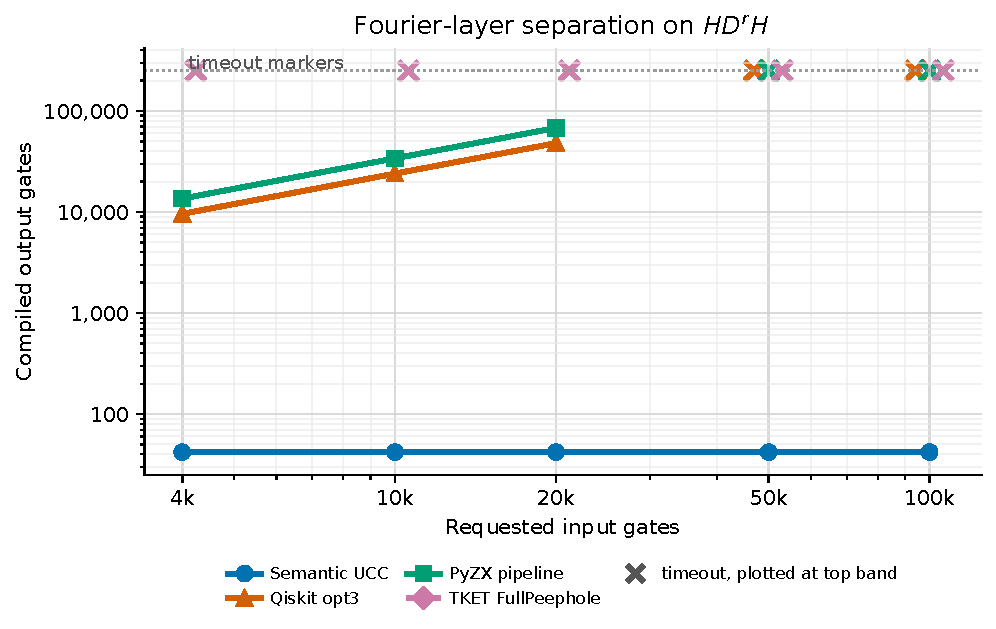
\includegraphics[width=0.95\linewidth]{figures/fourier_separation.pdf}
\caption{Fixed-width non-inverse Fourier-layer scaling on the $H D^r H$ witness. The semantic UCC path remains at the canonical $42$-gate output, while tested flat pipelines grow with requested size or time out under the fixed protocol.}
\label{fig:fourier-separation}
\end{figure}

These data should be read together with
\cref{fig:fourier-separation,tab:generalized-fourier-witness,thm:fourier-layer-separation,cor:fixed-width-fourier}.
The experimental family is the fixed-width regime of the theorem: the semantic
path aggregates the repeated commuting diagonal layer and emits a
constant-size circuit, while post-lowering baselines either grow with input
size or time out under the fixed protocol. The generalized suite shows that
this signature is stable across multiple diagonal topologies and angle
families at the same fixed width, including QFT-like dyadic angles and mixed
signed angles. The PyZX and TKET rows are not used as formal lower bounds on
those systems; they are empirical evidence that, in the canonical pipeline,
strong external tools did not recover the global diagonal representation that
the semantic theorem identifies as necessary.

\begin{table*}[t]
\centering
\scriptsize
\begin{tabular}{@{}>{\raggedright\arraybackslash}p{0.17\textwidth}
                >{\raggedright\arraybackslash}p{0.20\textwidth}
                >{\raggedright\arraybackslash}p{0.32\textwidth}
                >{\raggedright\arraybackslash}p{0.18\textwidth}@{}}
\toprule
Pipeline & Representation tested & Observed behavior on $H D^r H$ & Interpretation \\
\midrule
Semantic UCC path
& pre-basis Fourier-layer term
& $42$ gates, depth $24$, $12$ \texttt{cx} at every tested scale
& semantic side \\
\texttt{qiskit opt3}
& preset target-basis pipeline
& $9{,}588$, $23{,}988$, $47{,}988$ gates; timeout at $50$k and $100$k
& no global diagonal recovery in this protocol \\
Qiskit commutative inverse cancellation
& targeted inverse/commutation control
& $13{,}574$, $33{,}974$ gates at $4$k, $10$k; timeout from $20$k
& inverse cancellation is not the mechanism \\
PyZX pipeline
& Qiskit--QASM--PyZX--Qiskit algebraic stress test
& $13{,}574$, $33{,}974$, $67{,}974$ gates; timeout at larger sizes
& no global phase-polynomial recovery in this pipeline \\
TKET FullPeephole
& strong peephole-oriented external baseline
& timeout from $4$k under the fixed protocol
& bounded local/peephole side \\
No-Fourier UCC ablation
& same artifact with Fourier-layer semantic path disabled
& timeout at every tested scale in the ablation run
& semantic-path causality check \\
\bottomrule
\end{tabular}
\caption{External-pipeline failure matrix for the fixed-width Fourier-layer witness. The table is a representation diagnostic, not a universal ranking of compilers: a future implementation that reconstructs a global phase-polynomial, ZX, or commuting-diagonal IR belongs on the semantic side of the separation.}
\label{tab:external-failure-matrix}
\end{table*}

\subsubsection{Fourier-layer semantic-path ablation}

To test whether the $42$-gate output is caused by the Fourier-layer semantic
representation rather than by ordinary downstream pass ordering, we disable
the Fourier-layer IR path and rerun the fixed-width $H D^r H$ witness. The
result is summarized in \cref{tab:fourier-ablation} and visualized in
\cref{fig:fourier-ablation}. This is a mechanism ablation, not an
method-ranking comparison: the relevant comparison is between
Fourier-enabled UCC modes and the no-Fourier semantic-path variant.

\begin{table}[tbp]
\centering
\begin{tabular}{rllll}
\toprule
Requested & \texttt{qiskit opt3} & baseline UCC & semantic UCC & no Fourier-layer IR \\
\midrule
4{,}000 & 9{,}588 / 3.800 s & 42 / 7.862 s & 42 / 7.593 s & timeout $>60$ s \\
10{,}000 & 23{,}988 / 24.168 s & 42 / 33.269 s & 42 / 32.363 s & timeout $>60$ s \\
20{,}000 & timeout $>60$ s & timeout $>60$ s & timeout $>60$ s & timeout $>60$ s \\
50{,}000 & timeout $>120$ s & 42 / 76.554 s & 42 / 80.594 s & timeout $>120$ s \\
100{,}000 & timeout $>120$ s & 42 / 110.383 s & 42 / 110.816 s & timeout $>120$ s \\
\bottomrule
\end{tabular}
\caption{Fourier-layer semantic-path ablation on the fixed-width $H D^r H$ witness. Disabling Fourier-layer semantic IR removes successful constant-output recovery at all tested sizes. Fourier-enabled UCC modes return the canonical $42$-gate circuit whenever they complete. The $20$k row timed out for every method in this ablation run and is therefore retained as a runtime caveat rather than a quality comparison.}
\label{tab:fourier-ablation}
\end{table}

\begin{figure}[t]
\centering
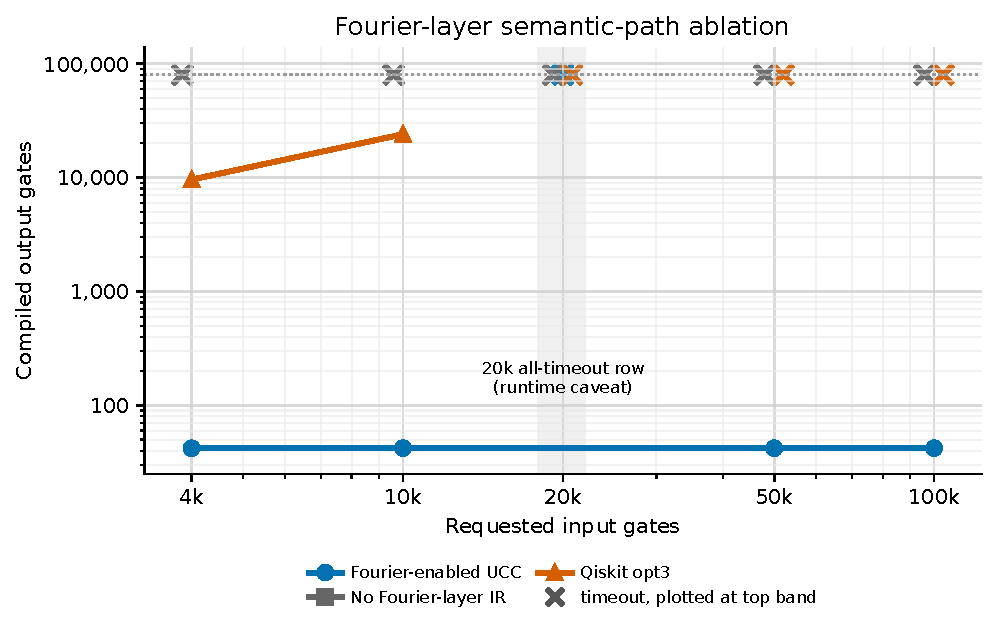
\includegraphics[width=0.95\linewidth]{figures/fourier_ablation.pdf}
\caption{Mechanism ablation for the fixed-width $H D^r H$ witness. Disabling the Fourier-layer semantic path removes completed constant-output recovery under the tested timeout budgets, while Fourier-enabled paths recover the canonical $42$-gate circuit whenever they complete.}
\label{fig:fourier-ablation}
\end{figure}

The ablation strengthens the causal interpretation of the Fourier-layer
result. In the no-Fourier variant, the compiler never recovers a completed
constant-size circuit under the timeout budget. In contrast, the
Fourier-enabled UCC paths recover the same $42$-gate canonical circuit whenever
they finish. Thus the constant form is tied to semantic Fourier-layer lifting
and coefficient aggregation, not merely to a favorable ordering of flat
post-lowering passes.

\subsubsection{Resource-consequence experiment}

The Fourier-layer separation is not only a gate-count phenomenon. To test
whether the same representation gap affects resource estimation, we compare a
semantic-first path against materialize-first paths on the
\texttt{fourier\_phase\_sandwich} family. The semantic-first path performs
Fourier-layer aggregation before target-basis materialization. The
materialize-first paths first lower or optimize the expanded circuit using
\texttt{qiskit opt3} or a no-Fourier-IR UCC path. We then count rotations and
estimate a Clifford+$T$ synthesis proxy
\[
T_{\epsilon}(R)
=
\left\lceil 3\log_2(1/\epsilon)\right\rceil R,
\]
where $R$ is the number of arbitrary \texttt{rx}/\texttt{ry}/\texttt{rz}
rotations. This is a reproducible synthesis-cost proxy, not an exact optimal
$T$ count.

\begin{table*}[t]
\centering
\footnotesize
\begin{tabularx}{\textwidth}{rXXX}
\toprule
Requested & semantic first & materialize-first \texttt{qiskit opt3} & materialize-first no-Fourier UCC \\
\midrule
4{,}000 & 42 / 12 / 22 / 2{,}200 & 9{,}588 / 4{,}788 / 4{,}793 / 479{,}300 & 9{,}588 / 4{,}788 / 4{,}793 / 479{,}300 \\
10{,}000 & 42 / 12 / 22 / 2{,}200 & 23{,}988 / 11{,}988 / 11{,}993 / 1{,}199{,}300 & timeout $>120$ s \\
20{,}000 & 42 / 12 / 22 / 2{,}200 & 47{,}988 / 23{,}988 / 23{,}993 / 2{,}399{,}300 & timeout $>600$ s \\
50{,}000 & 42 / 12 / 22 / 2{,}200 & timeout $>600$ s & timeout $>600$ s \\
100{,}000 & 42 / 12 / 22 / 2{,}200 & timeout $>600$ s & timeout $>600$ s \\
\bottomrule
\end{tabularx}
\caption{Resource-consequence experiment on the fixed-width $H D^r H$ witness. Each non-timeout cell reports gates / \texttt{cx} / rotations / $T_{10^{-10}}$ proxy. Semantic-first aggregation keeps all resource estimates constant, whereas materialize-first pipelines either grow linearly in the rotation and $T$-proxy estimates or time out.}
\label{tab:resource-consequence}
\end{table*}

\begin{figure}[t]
\centering
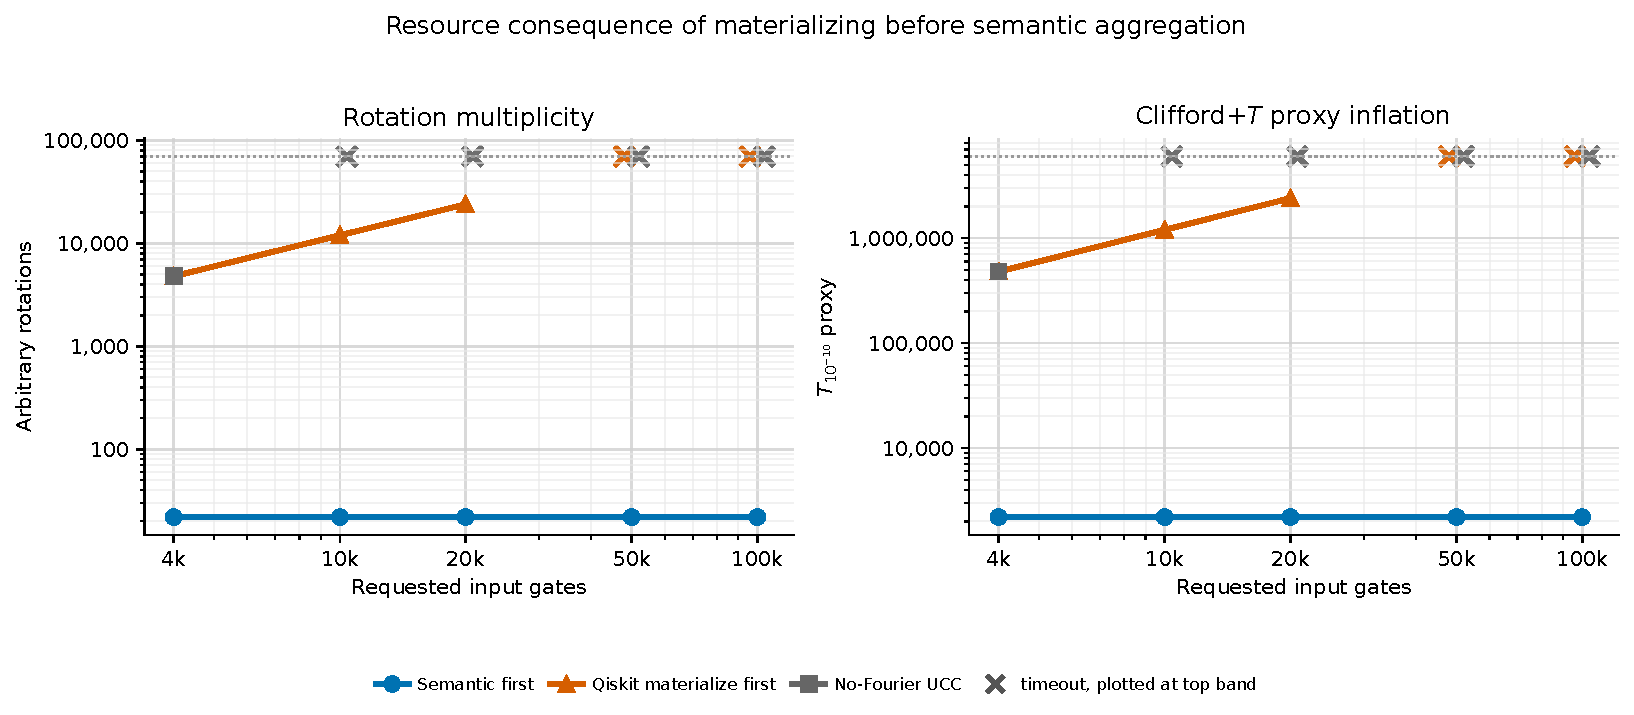
\includegraphics[width=0.95\linewidth]{figures/resource_consequence.pdf}
\caption{Resource-consequence view of the fixed-width Fourier-layer witness. Semantic-first aggregation keeps rotation and $T_{10^{-10}}$ proxy estimates constant, while materialize-first pipelines expose a linearly growing number of rotation tasks before timing out.}
\label{fig:resource-consequence}
\end{figure}

At precision $10^{-6}$ and $10^{-12}$ the same scaling holds: semantic-first
compilation stays at $T$-proxy values $1{,}320$ and $2{,}640$, respectively,
while materialize-first \texttt{qiskit opt3} reaches $1{,}439{,}580$ and
$2{,}879{,}160$ at $20$k before timing out at larger sizes. This experiment
therefore connects the recoverability theorem to a fault-tolerant compilation
concern: if coefficient aggregation is delayed until after basis
materialization, resource estimates can be inflated by the unrecovered
rotation multiplicity.

The physical point is the ordering of semantic aggregation relative to
synthesis. In a fault-tolerant pipeline, arbitrary rotations are eventually
approximated by discrete resources such as Clifford+$T$ sequences. If the
compiler first materializes $r$ separate rotations and only later estimates or
synthesizes them, the resource estimator sees $r$ independent approximation
tasks. A semantic-first pipeline instead combines the coefficients first and
presents one aggregated rotation per phase term. The proxy in
\cref{tab:resource-consequence,fig:resource-consequence} deliberately does not
model optimal number-theoretic synthesis or cancellation inside a synthesized
Clifford+$T$ sequence; it isolates the representation-level multiplicity that
enters any resource estimator before such backend-specific optimizations.
Thus the resource-consequence result should be read as an FTQC relevance
argument for pre-synthesis semantic aggregation, not as a claim of exact
optimal $T$ count.

\subsection{Why Simple Pass Reordering Is Not Enough}

To test whether the observed gains are mainly explained by a missing pass or
pass-ordering issue inside \texttt{UCCDefaults}, we ran a controlled comparison
between baseline UCC, several minimal \texttt{UCCDefaults}-style repairs, and the
semantic artifact. The minimal repair variants were
\texttt{defaults\_preinverse\_only}, \texttt{defaults\_reordered\_only}, and
\texttt{defaults\_minimal\_bundle}; the all-to-all cases were normalized to the
same final target basis $B = [\texttt{cx},\texttt{rx},\texttt{ry},\texttt{rz},\texttt{h}]$,
and the backend-aware cases used fixed transpiler seed $12345$. This is a
separate reorder-probe experiment, so its runtime numbers should be read
independently from the frozen mainline tables below.

\begin{table*}[t]
\centering
\scriptsize
\begin{tabular}{llrrrr}
\toprule
Case & Method & Gates & Depth & CX count & Runtime \\
\midrule
\multirow{6}{*}{\texttt{phase\_estimation\_real}}
  & baseline UCC & 471{,}819 & 328{,}271 & 81{,}906 & 75.538 s \\
  & \texttt{defaults\_preinverse\_only} & 485{,}780 & 332{,}924 & 82{,}925 & 80.045 s \\
  & \texttt{defaults\_reordered\_only} & 485{,}780 & 332{,}924 & 82{,}925 & 80.005 s \\
  & \texttt{defaults\_minimal\_bundle} & 485{,}780 & 332{,}924 & 82{,}925 & 80.084 s \\
  & semantic UCC & 166{,}805 & 119{,}204 & 27{,}303 & 1.989 s \\
  & \texttt{qiskit opt3} & 166{,}805 & 119{,}204 & 27{,}303 & 1.254 s \\
\midrule
\multirow{6}{*}{\texttt{qaoa\_ring\_100k}}
  & baseline UCC & 300{,}055 & 163{,}055 & 40{,}000 & 2.431 s \\
  & \texttt{defaults\_preinverse\_only} & 434{,}104 & 217{,}962 & 40{,}000 & 11.352 s \\
  & \texttt{defaults\_reordered\_only} & 445{,}216 & 217{,}962 & 40{,}000 & 10.120 s \\
  & \texttt{defaults\_minimal\_bundle} & 434{,}104 & 217{,}962 & 40{,}000 & 10.818 s \\
  & semantic UCC & 100{,}000 & 62{,}000 & 40{,}000 & 3.131 s \\
  & \texttt{qiskit opt3} & 100{,}000 & 62{,}000 & 40{,}000 & 0.307 s \\
\midrule
\multirow{6}{*}{\texttt{hw\_mqt\_qpeexact\_20}}
  & baseline UCC & 2{,}077 & 626 & 1{,}262 & 0.126 s \\
  & \texttt{defaults\_preinverse\_only} & 1{,}893 & 576 & 1{,}311 & 0.292 s \\
  & \texttt{defaults\_reordered\_only} & 1{,}900 & 582 & 1{,}312 & 0.289 s \\
  & \texttt{defaults\_minimal\_bundle} & 1{,}893 & 576 & 1{,}311 & 0.287 s \\
  & semantic UCC & 1{,}593 & 420 & 772 & 0.296 s \\
  & \texttt{qiskit opt3} & 1{,}572 & 407 & 812 & 0.033 s \\
\midrule
\multirow{6}{*}{\texttt{hw\_mqt\_qaoa\_20}}
  & baseline UCC & 2{,}088 & 522 & 1{,}439 & 0.098 s \\
  & \texttt{defaults\_preinverse\_only} & 2{,}050 & 487 & 1{,}458 & 0.270 s \\
  & \texttt{defaults\_reordered\_only} & 2{,}050 & 487 & 1{,}458 & 0.269 s \\
  & \texttt{defaults\_minimal\_bundle} & 2{,}050 & 487 & 1{,}458 & 0.271 s \\
  & semantic UCC & 2{,}050 & 487 & 1{,}458 & 0.278 s \\
  & \texttt{qiskit opt3} & 2{,}091 & 532 & 1{,}530 & 0.048 s \\
\bottomrule
\end{tabular}
\caption{Controlled comparison of baseline UCC, minimal \texttt{UCCDefaults}-style repairs, the semantic artifact, and \texttt{qiskit opt3}. Small default-pipeline fixes explain part of the improvement on some cases, but they do not account for the main gains on the real and structured workloads.}
\label{tab:defaults-vs-full}
\end{table*}

\cref{tab:defaults-vs-full} makes the conclusion more direct. Small
default-pipeline fixes explain only part of the behavior. On the real
algorithm-family instances, the minimal bundle remains far from the semantic
artifact: \texttt{phase\_estimation\_real} gives $485{,}780$ gates for
\texttt{defaults\_minimal\_bundle} versus $166{,}805$ for the semantic artifact
and \texttt{qiskit opt3}. The gap is also clear on large structured cases:
\texttt{qaoa\_ring\_100k} gives $434{,}104$ gates for the minimal bundle, while
the semantic artifact and \texttt{qiskit opt3} both return $100{,}000$. One
partial exception is \texttt{hw\_mqt\_qaoa\_20}, where the minimal bundle already
matches the semantic artifact. Even in the hardware-aware setting, however, the
reorder-only explanation is incomplete: on \texttt{hw\_mqt\_qpeexact\_20}, the
minimal bundle gives $1{,}893$ gates, depth $576$, and \texttt{cx} count
$1{,}311$, while the semantic artifact gives $1{,}593$, depth $420$, and
\texttt{cx} count $772$.

\subsection{Official Real Algorithm-Family Instances}

We evaluated the semantic artifact on three official Qiskit circuit-library instances under the fixed target basis $B = [\texttt{cx},\texttt{rx},\texttt{ry},\texttt{rz},\texttt{h}]$. The frozen-run results are shown in \cref{tab:real-instances}.

\begin{table}[h]
\centering
\begin{tabular}{lcccc}
\toprule
Instance & Method & Gates & Depth & Runtime \\
\midrule
\multirow{4}{*}{\texttt{phase\_estimation\_real}}
  & translation only & 159{,}838 & 121{,}214 & 0.100 s \\
  & qiskit opt3 & 166{,}805 & 119{,}204 & 1.298 s \\
  & baseline UCC & 471{,}819 & 328{,}271 & 80.923 s \\
  & semantic UCC & 166{,}805 & 119{,}204 & 1.364 s \\
\midrule
\multirow{4}{*}{\texttt{grover\_real}}
  & translation only & 85{,}403 & 55{,}892 & 0.084 s \\
  & qiskit opt3 & 79{,}029 & 54{,}163 & 0.552 s \\
  & baseline UCC & 287{,}047 & 152{,}298 & 1.915 s \\
  & semantic UCC & 79{,}029 & 54{,}163 & 0.556 s \\
\midrule
\multirow{4}{*}{\texttt{qaoa\_real}}
  & translation only & 36{,}512 & 2{,}416 & 0.020 s \\
  & qiskit opt3 & 36{,}512 & 2{,}416 & 0.272 s \\
  & baseline UCC & 167{,}833 & 7{,}133 & 1.010 s \\
  & semantic UCC & 36{,}512 & 2{,}416 & 0.273 s \\
\bottomrule
\end{tabular}
\caption{Frozen-run results on official real algorithm-family instances.}
\label{tab:real-instances}
\end{table}

These official real-instance experiments support the recoverability-parity
regime. Baseline UCC exhibits severe regressions on real algorithm-family
circuits, whereas the semantic artifact recovers the same output quality as
\texttt{qiskit opt3}. Relative to baseline UCC, the semantic artifact cuts gate
count by about $64.6\%$ on \texttt{phase\_estimation\_real}, $72.5\%$ on
\texttt{grover\_real}, and $78.2\%$ on \texttt{qaoa\_real}. The runtime gap to
\texttt{qiskit opt3} is also reduced to a small constant factor on all three
instances.

\begin{figure}[t]
\centering
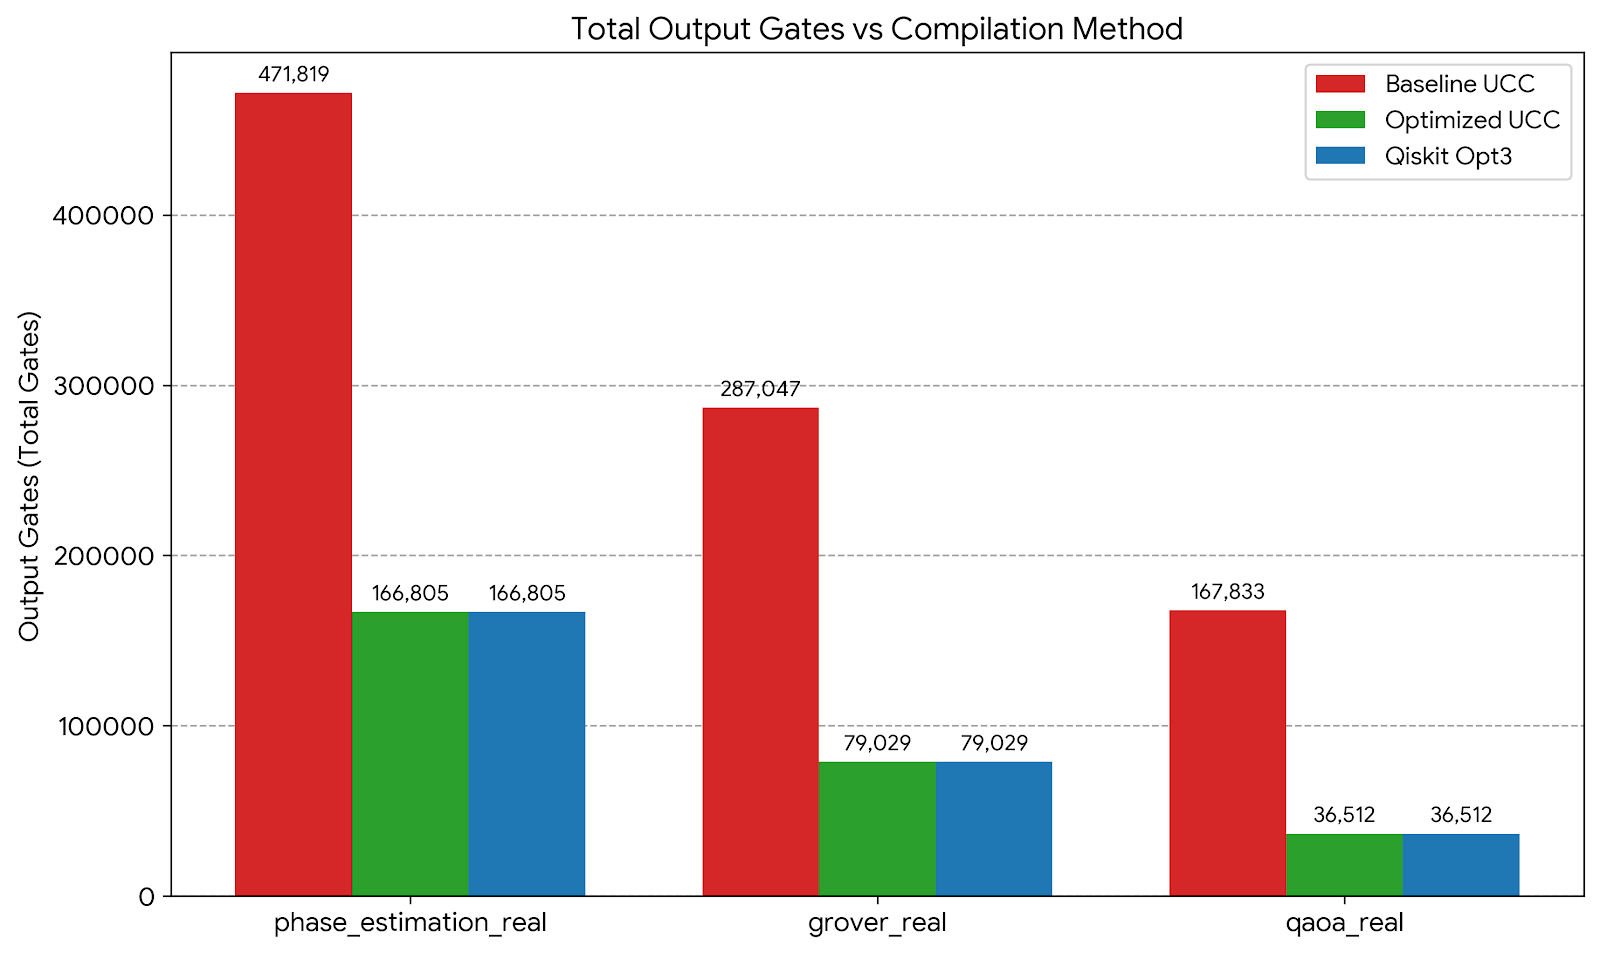
\includegraphics[width=0.95\linewidth]{figures/real_instance_grouped_bar.png}
\caption{Total output gate counts on the three official real instances. The semantic UCC artifact matches \texttt{qiskit opt3}-level output quality while substantially improving over baseline UCC.}
\label{fig:real-instance-bars}
\end{figure}

This quality-recovery pattern is also shown visually in
\cref{fig:real-instance-bars}: on all three official real instances, the
semantic artifact matches the output-gate quality of \texttt{qiskit opt3} while
substantially improving over baseline UCC.

\subsection{Public Benchmark Suite Results}

To move beyond official library examples, we added two public benchmark sources: \texttt{MQT Bench} and \texttt{SupermarQ}.

\paragraph{MQT Bench.}
Representative results are:
\begin{itemize}[leftmargin=1.5em]
    \item \texttt{mqt\_qpeexact\_32}: \texttt{qiskit opt3} $= 1{,}891$ gates, baseline UCC $= 5{,}494$, semantic UCC $= 1{,}891$;
    \item \texttt{mqt\_qpeinexact\_24}: \texttt{qiskit opt3} $= 1{,}206$ gates, baseline UCC $= 3{,}682$, semantic UCC $= 1{,}206$;
    \item \texttt{mqt\_ae\_8}: \texttt{qiskit opt3} $= 207$ gates, baseline UCC $= 542$, semantic UCC $= 207$;
    \item \texttt{mqt\_draper\_qft\_adder\_32}: \texttt{qiskit opt3} $= 1{,}630$ gates, baseline UCC $= 5{,}278$, semantic UCC $= 1{,}630$;
    \item \texttt{mqt\_qaoa\_32}: \texttt{qiskit opt3} $= 1{,}422$ gates, baseline UCC $= 6{,}310$, semantic UCC $= 1{,}422$;
    \item \texttt{mqt\_grover\_20}: \texttt{qiskit opt3} $= 3{,}848{,}810$ gates in $38.043$ s, baseline UCC times out at $>120$ s, and semantic UCC reaches the same output quality in $39.123$ s.
\end{itemize}
Thus, on \texttt{MQT Bench}, the semantic artifact repeatedly recovers
\texttt{qiskit opt3}-level output quality and clearly improves over baseline
UCC. The added \texttt{qpeinexact}, \texttt{ae}, and
\texttt{draper\_qft\_adder} cases are especially relevant because they extend
the phase-ladder/Fourier-layer story beyond one exact-QPE benchmark into
inexact QPE, amplitude estimation, and QFT-based arithmetic. Runtime still
remains weaker on the hardest Grover-style case.

Additional mirrored/conjugation positive cases make the second theory line more
concrete. On the official \texttt{grover\_real} instance, baseline UCC returns
$287{,}047$ gates while the semantic artifact and \texttt{qiskit opt3} both return
$79{,}029$. On \texttt{MQT Bench} Grover instances, the same pattern persists
across scale: \texttt{mqt\_grover\_8} gives $18{,}992 \rightarrow 5{,}170$,
\texttt{mqt\_grover\_12} gives $259{,}797 \rightarrow 71{,}706$, and
\texttt{mqt\_grover\_16} gives $2{,}112{,}285 \rightarrow 581{,}098$, where in
each case the semantic artifact exactly matches \texttt{qiskit opt3} while clearly
improving on baseline UCC. The large fixed-basis mirrored Grover benchmark shows
the same parity pattern: baseline UCC gives $4{,}122{,}006$ gates, while
the semantic artifact and \texttt{qiskit opt3} both give $1{,}158{,}011$. These cases make the
mirrored/conjugation line less dependent on the routed timeout-recovery
interpretation of \texttt{hw\_mqt\_grover\_20}.

A dedicated mirrored/conjugation scaling sweep makes this support more
systematic. On public \texttt{MQT Bench} Grover instances, the semantic artifact
matches \texttt{qiskit opt3} exactly at sizes $8$, $12$, and $16$, reducing
baseline UCC from $18{,}992$ to $5{,}170$ gates, from $259{,}797$ to $71{,}706$
gates, and from $2{,}112{,}285$ to $581{,}098$ gates, respectively. On the
fixed-basis \texttt{grover\_mirrored} repeated-shell scaling sweep, the same
parity pattern holds at $10$k, $20$k, $50$k, and $100$k input gates:
baseline UCC gives $412{,}206$, $824{,}406$, $2{,}061{,}006$, and
$4{,}122{,}006$ output gates, while the semantic artifact and \texttt{qiskit opt3}
give $115{,}811$, $231{,}611$, $579{,}011$, and $1{,}158{,}011$ gates. Thus
the second theory line is now supported by both public Grover scaling and
large repeated-shell fixed-basis scaling.

\paragraph{SupermarQ.}
Representative results are:
\begin{itemize}[leftmargin=1.5em]
    \item \texttt{supermarq\_mermin\_bell\_8}: baseline UCC $= 386$ gates, depth $135$; semantic UCC $= 76$ gates, depth $44$; \texttt{qiskit opt3} $= 76$ gates, depth $44$;
    \item \texttt{supermarq\_qaoa\_vanilla\_12}: baseline UCC $= 947$ gates, depth $225$; semantic UCC $= 222$ gates, depth $80$; \texttt{qiskit opt3} $= 222$ gates, depth $80$;
    \item \texttt{supermarq\_hamiltonian\_sim\_8}: baseline UCC $= 71$ gates, depth $36$; semantic UCC $= 51$ gates, depth $24$; \texttt{qiskit opt3} $= 51$ gates, depth $24$.
\end{itemize}
This second public benchmark source strengthens the paper in two ways. It shows clear anti-regression behavior on additional nontrivial families, and it also exposes a realistic limitation: the semantic artifact is not uniformly better on every benchmark family.

\subsection{Hardware-Aware Results}

We added a backend-aware comparison using a fixed $20$-qubit bidirectional line backend with native operations \texttt{u}, \texttt{sx}, \texttt{p}, \texttt{cx}, \texttt{measure}, and \texttt{id}. The benchmark source is \texttt{MQT Bench}, and the cases are \texttt{hw\_mqt\_qpeexact\_20}, \texttt{hw\_mqt\_qaoa\_20}, and \texttt{hw\_mqt\_grover\_20}.

\paragraph{\texttt{hw\_mqt\_qpeexact\_20}.}
\begin{table}[h]
\centering
\begin{tabular}{lrrrr}
\toprule
Method & Output Gates & Output Depth & CX Count & Runtime \\
\midrule
qiskit opt3 & 1{,}572 & 407 & 812 & 0.056 s \\
baseline UCC & 1{,}976 & 648 & 1{,}350 & 0.174 s \\
semantic UCC & 1{,}572 & 407 & 812 & 0.235 s \\
\bottomrule
\end{tabular}
\caption{Hardware-aware results for \texttt{hw\_mqt\_qpeexact\_20}.}
\label{tab:hw-qpe}
\end{table}

This is a clean fixed-seed parity case: the semantic artifact matches
\texttt{qiskit opt3} in total gates, depth, and \texttt{cx} count, while still
remaining much better than baseline UCC on all structural metrics. The tradeoff
is runtime rather than output quality.

\paragraph{\texttt{hw\_mqt\_qaoa\_20}.}
\begin{table}[h]
\centering
\begin{tabular}{lrrrr}
\toprule
Method & Output Gates & Output Depth & CX Count & Runtime \\
\midrule
qiskit opt3 & 2{,}091 & 532 & 1{,}530 & 0.078 s \\
baseline UCC & 2{,}057 & 513 & 1{,}503 & 0.141 s \\
semantic UCC & 2{,}050 & 487 & 1{,}458 & 0.112 s \\
\bottomrule
\end{tabular}
\caption{Hardware-aware results for \texttt{hw\_mqt\_qaoa\_20}.}
\label{tab:hw-qaoa}
\end{table}

This is the clearest hardware-aware external-baseline win in the paper: the
semantic artifact improves on \texttt{qiskit opt3} in total gates, depth, and
\texttt{cx} count, while also improving on baseline UCC in total gates, depth,
and \texttt{cx} count.

\paragraph{\texttt{hw\_mqt\_grover\_20}.}
\texttt{qiskit opt3} and baseline UCC still time out under this setting,
but the semantic artifact returns a result in 1.999\,s via a stronger
mirrored/self-inverse repeated-run backend fallback. The resulting circuit is
still extremely large, but the selector lowers total gates, depth, and
\texttt{cx} simultaneously (to $6{,}467{,}857$ total gates, depth
$4{,}094{,}196$, and \texttt{cx} count $3{,}045{,}048$), so we treat this as a
robustness result rather than a main competitive routed-quality claim.

\subsection{Stability and Seed Sensitivity}

We measured repeated-run stability on the frozen artifact in two ways:
\begin{enumerate}[leftmargin=1.5em]
    \item five repeated runs for the official real instances and the canonical hardware-aware seed,
    \item a five-seed sweep for the backend-aware \texttt{MQT Bench} cases.
\end{enumerate}

The main conclusions are:
\begin{itemize}[leftmargin=1.5em]
    \item the official real-instance outputs are deterministic across repeated runs,
    \item the hardware-aware outputs are deterministic for each fixed seed,
    \item \texttt{hw\_mqt\_qaoa\_20} remains a win over \texttt{qiskit opt3} across all five tested seeds $0$, $1$, $42$, $12345$, and $54321$,
    \item \texttt{hw\_mqt\_qpeexact\_20} is now a fixed-seed parity case rather than a clean win.
\end{itemize}
Thus, the hardware-aware claim is a stable workload-family result across a small
fixed seed portfolio, rather than a single favorable seed.

\subsection{Runtime Engineering Progress}

The runtime story improved materially through three engineering changes: a direct Qiskit-source fast path for suitable all-to-all composite circuits, selective backend portfolio expansion, and backend reference pruning. These changes preserve the important quality results while substantially reducing avoidable overhead.

For the official real instances, the semantic artifact now runs much closer to
direct \texttt{qiskit opt3} than earlier versions. In the latest runtime-focused
comparisons, the all-to-all gap becomes very small on
\texttt{phase\_estimation\_real}, reaches parity on \texttt{grover\_real}, and
flips in favor of the semantic artifact in one profiling run on
\texttt{qaoa\_real}. On the hardware-aware side, pruning reduces runtime on
\texttt{hw\_mqt\_qpeexact\_20} and \texttt{hw\_mqt\_qaoa\_20} while preserving the
key quality outcomes, especially the external-baseline win on
\texttt{hw\_mqt\_qaoa\_20}. We treat these profiling results as engineering
support rather than as main paper claims; the canonical quantitative claims
remain the frozen summary tables above.

\begin{figure*}[t]
\centering
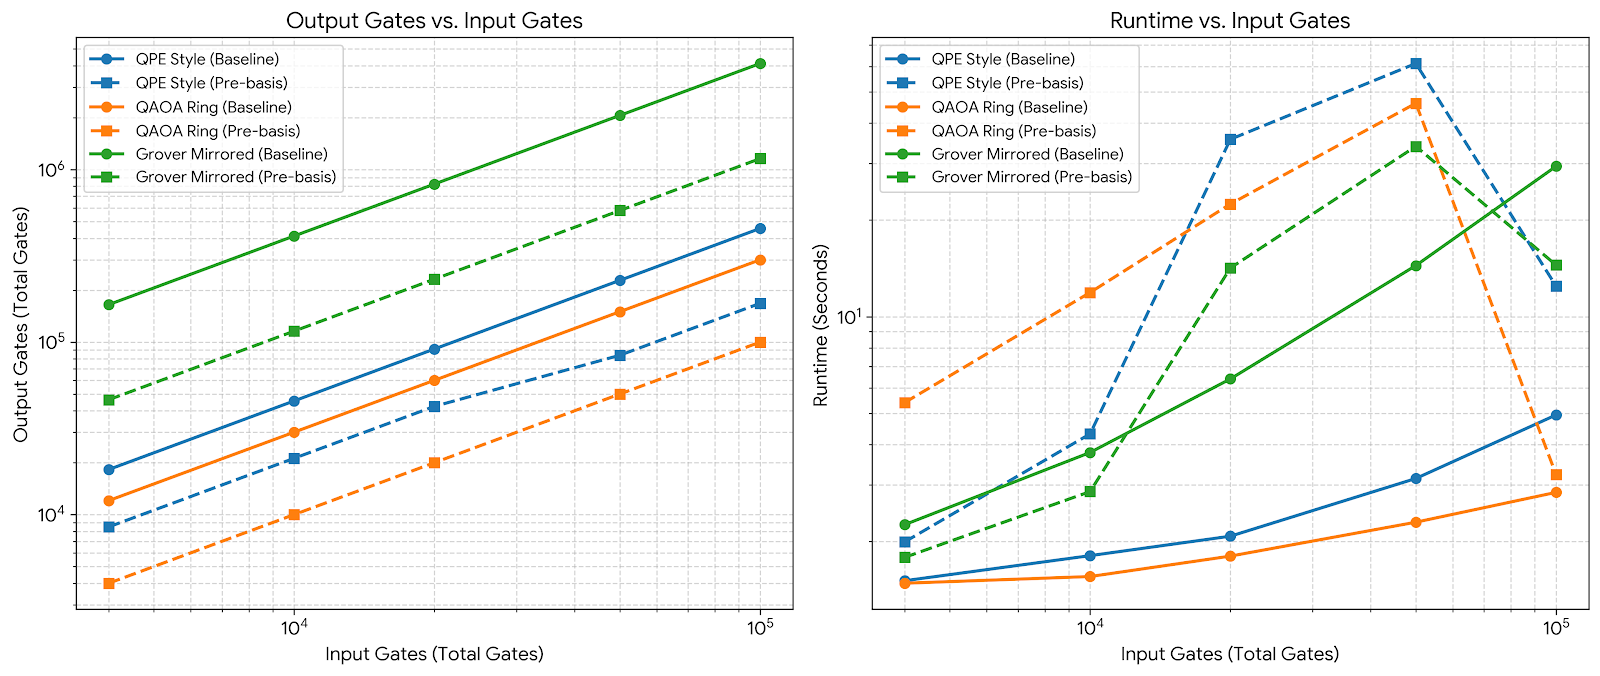
\includegraphics[width=\textwidth]{figures/scaling_plot.png}
\caption{Scaling behavior on representative structured families. Left: output gate count versus input gate count for baseline UCC and the semantic UCC artifact. Right: runtime versus input gate count. The semantic path preserves clear quality advantages across scale, while runtime behavior remains family-dependent.}
\label{fig:scaling}
\end{figure*}

\subsection{Scaling and Ablation}

The main scaling trends are summarized in \cref{fig:scaling}. The size sweep
covers $4$k, $10$k, $20$k, $50$k, and $100$k inputs for QFT-inverse,
QPE-style, QAOA-ring, and mirrored-Grover families. The most important
observations are stable quality behavior across scale and improving
repeated-family runtime once the semantic IR and dispatch controller are
enabled. The method is most effective on exact or highly repeated structure:
\texttt{qft\_inverse} remains maximally strong across all tested sizes,
\texttt{qpe\_style} remains a strong positive fixed-basis case,
\texttt{qaoa\_ring} consistently avoids UCC inflation, and the mirrored-Grover
family continues to match Qiskit quality at $100$k while remaining
more expensive. Direct spot checks on the semantic artifact give
\texttt{qpe\_style} $=82{,}200$ gates at $50$k in $2.504$ s and $164{,}400$
gates at $100$k in $4.636$ s, reflecting the phase-ladder plus
repeated-run controller improvements.

The refreshed ablation picture is narrower than in the earliest draft. The dominant practical component is now conservative candidate control on recoverability-sensitive families, most clearly on \texttt{qaoa\_ring}, where the full configuration returns $10{,}000$ gates while the no-candidate-selection variant returns $30{,}055$. By contrast, \texttt{qft\_inverse}, \texttt{qft\_control}, \texttt{qpe\_style}, and \texttt{grover\_mirrored} are much less sensitive to the removal of individual structural rules than they were in the earlier artifact. This reinforces the paper's current framing: the main contribution is a bounded semantic representation and dispatch controller that preserve recoverability before flat materialization, rather than a single local identity.

\section{Discussion}
\label{sec:discussion}

The formal definitions above are intentionally restricted. They do not attempt
to characterize all useful quantum-circuit structure or to prove global
optimality. Instead, they isolate a representation-dependent obstruction:
after basis materialization, the local certificates available to a bounded
compiler can collide across many repeated interior positions. The theorem and
artifact should therefore be read as a statement about recoverability under a
representation constraint, not as a ranking of all possible compiler designs.

\subsection{Principle Exposed by the Separation}

The Fourier-layer result identifies a general compilation principle. If an
optimization consists of aggregating coefficients attached to a commuting
semantic object, then the representation that still names the object can be
asymptotically more powerful than a representation that has already expanded it
into a repeated target-basis stream. The unitary is the same in both
representations; the recoverable certificates are different.

This distinction is stronger than a pass-ordering observation. Pass ordering
can explain some UCCDefault regressions, and the paper explicitly treats
mirrored/conjugation cases as parity recovery when strong flat baselines also
find the same simplification. The fixed-width Fourier witness plays a
different role: it removes inverse cancellation, isolates commuting diagonal
aggregation, and exhibits the predicted $\Omega(r)$ versus $O(1)$ behavior.

\subsection{Falsifiability}

The claim is deliberately falsifiable. A flat-stream pipeline that recovered
the constant Fourier form without constructing a global phase-polynomial, ZX,
stabilizer-phase, or commuting-diagonal representation would challenge the
restricted class as a model of practical flat recovery. A pipeline that
succeeds by constructing one of those representations would support the
semantic side of the separation. This is the intended boundary: the theorem
separates representation regimes, not brand names.

\subsection{Significance for Fault-Tolerant Synthesis}

The recoverability gap also has implications for fault-tolerant quantum
computing (FTQC), although the present experiments use fixed finite target
bases rather than a full fault-tolerant synthesis stack. In FTQC settings, a
dominant cost is often the synthesis of arbitrary rotations into a discrete
gate set such as Clifford+$T$. After such synthesis, the original rotation
coefficient may be much harder to recover from the discrete gate sequence.

The Fourier-layer theorem isolates the same kind of ordering issue at the
compiler-representation level. If repeated coefficients are aggregated before
lowering, the compiler lowers one semantic rotation with coefficient
$r\theta$; if the circuit is fully materialized first, recovering that global
coefficient may require a representation lift that bounded local rewriting
does not provide. This suggests that representation-aware preprocessing should
be treated as part of reliable resource estimation and synthesis pipelines, not
only as an engineering shortcut for NISQ-era circuits.

\Cref{tab:resource-consequence} makes this implication operational. Under the
rotation-count $T_{\epsilon}$ proxy, semantic-first compilation keeps the
fixed-width Fourier witness at $22$ rotations and a constant $T_{10^{-10}}$
proxy of $2{,}200$ across all tested sizes. A materialize-first
\texttt{qiskit opt3} path grows to $23{,}993$ rotations and a $T_{10^{-10}}$
proxy of $2{,}399{,}300$ at $20$k before timing out at $50$k and $100$k. The
numbers should not be read as exact optimal Clifford+$T$ counts; they show the
resource-estimation consequence of preserving or destroying the semantic
rotation multiplicity before synthesis.

\subsection{Synthesis of the Evidence}

The results support a single representation claim. Basis lowering can preserve
unitary semantics while destroying the bounded local evidence needed to recover
global Fourier-layer structure. The $H D^r H$ family is the primary witness:
semantic phase aggregation gives a fixed-width $\Omega(r)$ versus $O(1)$
separation, and the corresponding experiments exhibit the same
repetition-independent output signature against the tested flat pipelines. The
new generalized witness suite strengthens this point: across $42$ comparable
fixed-width topology/angle/scale points, semantic UCC wins structurally against
\texttt{qiskit opt3} in every case, while the semantic output remains tied to
the diagonal term structure rather than to the repetition count.

The ablation and resource-consequence experiments identify the mechanism. When
the Fourier-layer semantic path is disabled, completed constant-output recovery
disappears under the tested timeout budgets. When the semantic path is kept,
the artifact preserves the aggregated rotation multiplicity before
materialization, keeping the rotation-count and $T_{10^{-10}}$ proxy constant
on the fixed-width witness. The separation is therefore not merely a smaller
gate-count table; it is a representation effect that propagates into
synthesis-oriented resource estimates.

The broader benchmarks define scope. Mirrored/conjugation workloads provide
secondary evidence for recoverability-aware compilation: semantic lifting
prevents severe baseline-UCC regressions and restores parity on Grover-like and
mirrored-shell workloads. Official Qiskit instances, \texttt{MQT Bench}, and
\texttt{SupermarQ} show that this anti-regression behavior appears beyond the
minimal witness, while mixed runtime and parity cases show that the semantic
path is selective rather than uniformly dominant.

The most important negative result is also part of the claim boundary. Simple
pass-ordering fixes explain part of the UCCDefault behavior, but they do not
explain the fixed-width Fourier-layer separation, which requires preserving and
aggregating a semantic diagonal representation before flat materialization.
Conversely, any compiler that reconstructs a global phase-polynomial, ZX, or
commuting-diagonal representation should be classified on the semantic side of
the theorem. The contribution is therefore a representation boundary for
recoverability, with UCC serving as the artifact through which that boundary is
measured.

\section{Threats to Validity}
\label{sec:threats}

This study has several limitations.
\begin{enumerate}[leftmargin=1.5em]
    \item The theorem is a restricted-class separation, not a lower bound against all possible quantum compilers. A compiler that reconstructs a global phase-polynomial, ZX, or commuting-diagonal IR belongs to the semantic side of the separation.
    \item The fixed-width $H D^r H$ family is intentionally structured. It is a minimal theorem witness, not a claim that all QFT or QPE instances exhibit the same $\Omega(r)$ gap. The generalized witness suite varies topology and angle family at $n=4$, but it is not yet a width-scaling experiment.
    \item The external-baseline evidence is pipeline-specific. PyZX and TKET are evaluated through the artifact's QASM/Qiskit conversion and fixed-basis protocol, so their failure to recover the constant form is evidence about this configured pipeline rather than a theorem about those tools in all modes.
    \item The evaluation is centered on UCC and Qiskit-flavored workflows.
    \item The method is bounded and heuristic rather than globally optimal.
    \item Strong external baselines may still match or exceed the method on some families; mirrored and conjugation cases are therefore framed as parity recovery rather than primary separation evidence.
    \item The source-level short-circuit path depends on Qiskit-native all-to-all composite inputs and may not transfer unchanged to other frontend representations or compiler stacks.
    \item The hardware-aware stability evidence covers only a finite fixed seed portfolio and one chosen backend family, so it should not be read as a guarantee of robustness across all transpiler randomness or hardware settings.
    \item The Fourier ablation is a mechanism check for semantic Fourier lifting. Disabling the Fourier-layer IR path times out at every tested scale, while Fourier-enabled UCC modes recover the $42$-gate form whenever they complete. Since multiple Fourier-enabled modes can return the same canonical output, the conclusion is about semantic Fourier recognition broadly rather than one specific artifact shortcut. The generalized suite extends the structural-quality evidence, but the ablation was run on the canonical full-pair witness.
    \item The resource-consequence experiment uses a rotation-count proxy for Clifford+$T$ synthesis cost at fixed precision, rather than exact optimal synthesis. It supports the scaling consequence of delayed semantic aggregation, not a claim about optimal $T$ counts for every synthesis backend.
\end{enumerate}

\section{Reproducibility}
\label{sec:reproducibility}

The frozen research directory includes a standardized artifact entry point
(\path{run_frozen_artifact.py}), an environment snapshot, an output manifest,
and a reproducibility guide. Together these documents specify the local software
environment, the expected baseline and experimental repository layout, the
canonical output files for each experiment bundle, and the one-command
reproduction path for the frozen experiment suite.

The artifact package includes the frozen summary tables, raw JSON outputs,
markdown summaries, and the scripts needed to regenerate the principal figures
and tables used in the paper. For review, the artifact is organized so that each
paper figure and table can be traced back to its generating script and frozen
output files.

\section{Conclusion}
\label{sec:conclusion}

This paper identifies a representation-dependent recoverability gap in
structured quantum circuit compilation. Basis lowering can preserve unitary
semantics while removing the bounded local evidence needed to recover global
Fourier-layer and conjugation structure. The primary result is the
Fourier-layer recoverability separation: bounded flat recovery retains
$\Omega(rm)$ phase-gadget structure on $H_{\Lambda}D_m^rH_{\Lambda}$, whereas
semantic coefficient aggregation emits $O(m)$ structure and $O(1)$ structure in
the fixed-width case.

The UCC artifact makes this distinction operational. The canonical Fourier
witness gives a strict separation from tested flat pipelines, the generalized
fixed-width sweep shows the same repetition-independent semantic behavior
across topology and angle-family axes, the Fourier ablation ties the constant
output to semantic lifting, and the resource-consequence experiment shows how
the same representation gap can inflate rotation-count synthesis proxies.
Mirrored/conjugation families show the secondary anti-regression role of
semantic lifting by restoring parity on Grover-like workloads. The remaining
challenge is to broaden these recoverability gains beyond the present workload
families and to characterize more precisely which practical pipelines belong on
the flat-recovery side or the semantic-lifting side of the separation.

\begin{thebibliography}{10}

\bibitem{duncan2020zx}
Ross Duncan, Aleks Kissinger, Simon Perdrix, and John van de Wetering.
\newblock Graph-theoretic simplification of quantum circuits with the ZX-calculus.
\newblock {\em Quantum}, 4:279, 2020.

\bibitem{martiel2022lazy}
Simon Martiel and Timoth{\'e}e Goubault de Brugière.
\newblock Architecture aware compilation of quantum circuits via lazy synthesis.
\newblock {\em Quantum}, 6:729, 2022.

\bibitem{quetschlich2023mqtbench}
Nils Quetschlich, Lukas Burgholzer, and Robert Wille.
\newblock MQT Bench: Benchmarking software and design automation tools for quantum computing.
\newblock {\em Quantum}, 7:1062, 2023.

\bibitem{mills2021holistic}
Daniel Mills, Seyon Sivarajah, Travis L. Scholten, and Ross Duncan.
\newblock Application-motivated, holistic benchmarking of a full quantum computing stack.
\newblock {\em Quantum}, 5:415, 2021.

\bibitem{steiger2018projectq}
Damian S. Steiger, Thomas H{\"a}ner, and Matthias Troyer.
\newblock ProjectQ: an open source software framework for quantum computing.
\newblock {\em Quantum}, 2:49, 2018.

\bibitem{kreppel2023shuttling}
Fabian Kreppel, Christian Melzer, Diego Olvera Millán, Janis Wagner, Janine Hilder, Ulrich Poschinger, Ferdinand Schmidt-Kaler, and André Brinkmann.
\newblock Quantum circuit compiler for a shuttling-based trapped-ion quantum computer.
\newblock {\em Quantum}, 7:1176, 2023.

\bibitem{tan2024dpqa}
Daniel Bochen Tan, Dolev Bluvstein, Mikhail D. Lukin, and Jason Cong.
\newblock Compiling quantum circuits for dynamically field-programmable neutral atoms array processors.
\newblock {\em Quantum}, 8:1281, 2024.

\bibitem{watkins2024surfacecode}
George Watkins, Hoang Minh Nguyen, Keelan Watkins, Steven Pearce, Hoi-Kwan Lau, and Alexandru Paler.
\newblock A high performance compiler for very large scale surface code computations.
\newblock {\em Quantum}, 8:1354, 2024.

\bibitem{fellousasiani2023mnr}
Marco Fellous-Asiani, Jing Hao Chai, Yvain Thonnart, Hui Khoon Ng, Robert S. Whitney, and Alexia Auffèves.
\newblock Optimizing resource efficiencies for scalable full-stack quantum computers.
\newblock {\em PRX Quantum}, 4(4):040319, 2023.

\end{thebibliography}

\end{document}
